\documentclass[../main.tex]{subfiles}
\graphicspath{{../figures/}}

\usepackage{bm}
\usepackage[ntheorem]{empheq}
\usepackage[linesnumbered,ruled,vlined,resetcount,algochapter]{algorithm2e}
\usepackage{rotating}

\begin{document}

\mychapter{跨异构搜索空间的进化迁移神经架构搜索}
\label{sec:ch4-evolutionary-transfer-nas-heterogeneous-spaces}

\mysection{引言}
\label{sec:ch4-1-introduction}

如第一章所述,深度神经网络架构的设计对于模型性能至关重要,然而传统的人工设计或独立的NAS过程往往伴随着高昂的计算成本与经验难以复用的问题,构成了结构承载环节的主要效率瓶颈。虽然TNAS旨在通过复用先前任务的搜索经验来提升效率,但现有方法大多局限于在相同或相似的架构搜索空间(即同构空间)内进行迁移(见 1.2.2 节)。当面临源域与目标域的架构范式存在本质差异(即异构搜索空间)时,有效的知识迁移机制仍然阙如。这一挑战正是本章研究的核心切入点,直接回应了第一章(1.4.1 节)提出的核心科学问题 Q2。

本章聚焦于结构层面的知识迁移,旨在突破异构搜索空间的壁垒,提出一种名为 \textsc{Bridge} (Building Representation Inter-Domain Heterogeneous Evolutionary TNAS) 的新型跨域进化迁移神经架构搜索框架。\textsc{Bridge} 的核心思想并非直接迁移架构的句法结构,而是通过学习架构的统一语义表示,并在该表示空间中构建跨域映射,实现基于语义对齐的知识迁移。具体而言,我们将首先利用表示学习技术(详见 4.6 节),将来自不同搜索空间的神经网络架构编码为统一的、结构感知的潜在向量表示。随后,在这些表示空间之间学习一个结构保持的映射函数(详见 4.7 节),以桥接异构域之间的差异。最终,利用该表示与映射,我们将源域中已发现的高性能架构解有效地迁移至目标域,作为进化搜索(详见 4.8 节)的高质量初始种群,从而显著加速目标域的 NAS 过程并提升结果质量。

本章将详细阐述 \textsc{Bridge} 框架的设计原理、关键技术组件(包括架构分词器、基于 Transformer 的变分自编码器、跨域映射学习、进化序贯迁移优化策略 ESTO)及其实现细节。最后,我们将通过在一系列复杂度递增的搜索空间(包括 NAS-Bench-101, NAS-Bench-201, DARTS)上的大量实验,系统性地验证 \textsc{Bridge} 框架在实现跨异构搜索空间知识迁移、降低 NAS 成本以及发现高性能架构方面的有效性与优越性。

\mysection{问题背景与研究动机}
\label{sec:ch4-2-problem-background-and-motivation}

正如绪论(第一章)所阐述,神经架构搜索作为自动化模型设计的关键技术,虽取得了显著进展,但其高昂的计算成本以及架构知识难以跨任务复用的问题,依然是制约其广泛应用的主要障碍 。可迁移 NAS旨在通过复用先前任务的搜索经验来缓解此问题,然而现有 TNAS 方法大多局限于源域与目标域共享相同或相似架构定义的同构搜索空间内 。当面临的场景需要跨越不同的架构范式时——例如,将卷积神经网络的设计经验应用于 Transformer 架构的搜索,或将在小数据集上优化的浅层网络知识迁移至需要更深、更复杂网络的大数据集任务——即在异构搜索空间之间进行迁移时,现有 TNAS 方法往往因架构表示不兼容而失效 。

这种在异构搜索空间之间实现有效架构知识迁移的挑战,正是本章研究工作所要解决的核心问题,其背后蕴含着一系列独特的困难,也构成了驱动本文提出 \textsc{Bridge} 框架的直接动机:

首先,核心的障碍在于架构表示的异质性与不兼容性 。不同的搜索空间往往采用截然不同的设计语言来描述架构,包括不同的基础操作符集合(如卷积 vs 自注意力)、不同的连接拓扑规则(如 Cell-based DAG vs 全局连接)、以及不同的编码方式(如 OON vs OOE)。这导致源域中的一个架构 $a^{(S)}$ 无法直接翻译或映射为目标域中的一个有效架构 $a^{(T)}$。缺乏统一的表示框架,使得跨越异构空间的架构比较、关联和知识传递变得极其困难。因此,一个关键的研究动机在于:能否学习一种通用的、与具体搜索空间解耦的架构潜在表示,将不同范式的架构映射到同一个共享的语义空间中,从而为知识迁移搭建桥梁?

其次,即使能够建立统一表示,跨域性能关联的不确定性也构成了严峻挑战 。一个在源域任务和架构空间中表现优异的架构(或其表示),迁移到目标域后其性能如何,往往难以直接预测。任务目标、数据集特性以及架构空间本身的差异都可能导致性能关联发生变化。简单地将在源域中性能最优的架构直接迁移至目标域,未必能获得最佳结果。因此,另一个关键的研究动机在于:如何有效地建模和利用跨域的性能信息,以指导迁移过程? 这可能需要学习一个能够预测架构在目标域相对性能的代理模型,或者学习一个能够将源域表示映射到目标域中性能相当区域的跨域映射函数。

最后,直接或生硬的架构迁移极易引发负迁移的风险。由于源域和目标域的最优架构可能存在结构上的显著差异,从源域迁移过来的架构(即使经过表示空间的映射转换)在目标域中可能并非最优,甚至性能不佳。若迁移策略过于僵化,强行将源域知识施加于目标域搜索,反而可能限制了对目标域更优架构的探索。因此,第三个关键的研究动机在于:如何设计一种灵活且自适应的迁移策略,能够在有效利用源域知识(例如,提供高质量的搜索起点)的同时,允许架构在目标域中进行必要的调整和优化,以适应新的任务需求,从而最大限度地规避负迁移? 进化算法等基于种群的优化策略,因其固有的探索与适应能力,为实现这种适应性迁移提供了有前景的途径 。

综上所述,实现跨异构搜索空间的有效神经架构知识迁移,迫切需要解决架构表示的统一性、跨域性能关联的建模以及迁移策略的适应性这三大核心挑战。正是这些挑战共同构成了本章的研究动机,并直接导向了本文所提出的 \textsc{Bridge} 框架的核心设计思想:通过构建统一的架构表示学习机制(应对挑战一),结合基于性能排序的跨域映射学习(应对挑战二),并最终将迁移的知识融入进化优化框架(应对挑战三),以期实现高效、鲁棒且自适应的跨异构搜索空间神经架构搜索。

\mysection{相关研究综述}
\label{sec:ch4-3-related-work-review}

深度模型结构层面的自动化设计与迁移优化已成为研究热点。第一章(1.2.2 节)已对传统神经架构搜索的主流方法(如基于强化学习、进化算法、梯度优化和代理模型等)以及旨在复用架构经验的可迁移 NAS进行了系统性回顾。然而,正如前文所强调,现有 TNAS 的研究成果大多局限于同构搜索空间内的知识迁移 。本章的核心挑战在于突破这一限制,实现跨越不同架构范式和定义的\textbf{异构搜索空间}之间的有效知识迁移。因此,本节的相关工作综述将不再重复介绍基础 NAS 或同构 TNAS,而是\textbf{高度聚焦于直接针对跨异构 NAS 探索以及支撑此类迁移的关键技术——神经架构表示学习}的相关前沿工作。

目前,直接探讨跨异构搜索空间 NAS 的研究尚处于起步阶段,相关工作非常有限 。Yu Liu 等人在 NeurIPS 2022 提出的跨域预测器(Cross-Domain Predictor, CDP)是少数直接尝试应对此挑战的工作之一 。CDP 的核心思想并非直接迁移架构本身,而是试图训练一个能够在源域和目标域(即使架构空间不同)之间通用的性能预测模型。它利用领域自适应技术,将源空间和目标空间的架构(通过某种特征提取方式)投射到一个共享的特征空间,并在此空间训练性能预测器。其目标是实现“跨空间的性能度量”,从而在目标域 NAS 时,能够借助源域的性能数据来辅助评估,提高搜索效率 。然而,CDP 方法存在明显局限:首先,它仍依赖于源、目标空间在表示上具有一定的可比性或相似性,以便特征能够有效对齐;其次,CDP 仅提供了一个性能评估工具,并未给出如何将源域的优秀架构直接迁移或转化为目标域候选解的方案,目标空间的架构仍需独立搜索产生 。因此,CDP 更像是 NAS 的一种辅助加速手段,而非完整的跨异构迁移解决方案。

除了 CDP 之外,鲜有文献直接研究如何在不同架构范式之间进行设计经验的显式迁移 。这一研究空白凸显了当前领域面临的挑战,同时也预示着巨大的机遇。要实现跨异构空间的架构知识迁移,一个关键的前提是需要一种能够统一表示不同类型架构的机制。近年来,神经架构表示学习 的研究为此提供了有前景的方向 。其核心目标是学习一个从离散的、图状的架构空间到连续的、低维向量空间的映射(即编码器),使得架构在潜在表示空间中能够被方便地比较、插值和操作。例如,有工作提出将神经网络架构视为图结构,并利用图神经网络或 Transformer 等模型来学习其向量嵌入 。Lukasik 等人提出的平滑变分图嵌入方法,利用变分自编码器将架构嵌入到向量空间,并在此空间进行高效优化 。Yan 等人则研究了无监督的架构表示学习,证明了良好的表示有助于预测架构性能并加速 NAS 。这些工作表明,通过学习一个恰当的、能够捕捉架构关键结构与语义信息的潜在表示空间,有可能弥合不同搜索空间之间的语言障碍。

本文提出的 \textsc{Bridge} 框架正是在这一背景下,试图将统一的架构表示学习与显式的跨域解迁移相结合,以解决跨异构 TNAS 的核心难题。与 CDP 仅关注性能预测不同,\textsc{Bridge} 旨在学习一个共享的潜在表示空间,并在该空间中学习跨域映射函数,从而能够将源域的优秀架构解直接转化为目标域的高质量初始候选。进一步地,通过将这种显式迁移的解融入进化优化框架,\textsc{Bridge} 实现了知识利用与适应性探索的结合。因此,相较于现有有限的探索,\textsc{Bridge} 提供了一种更完整、更直接的跨异构搜索空间神经架构知识迁移解决方案。

\mysection{跨空间进化可迁移 NAS 框架}
\label{sec:ch4-4-transferable-evolutionary-nas-framework}

\begin{figure}[htbp]
	\centering
	\typeout{Including: \textsc{Bridge}/overview.pdf}
	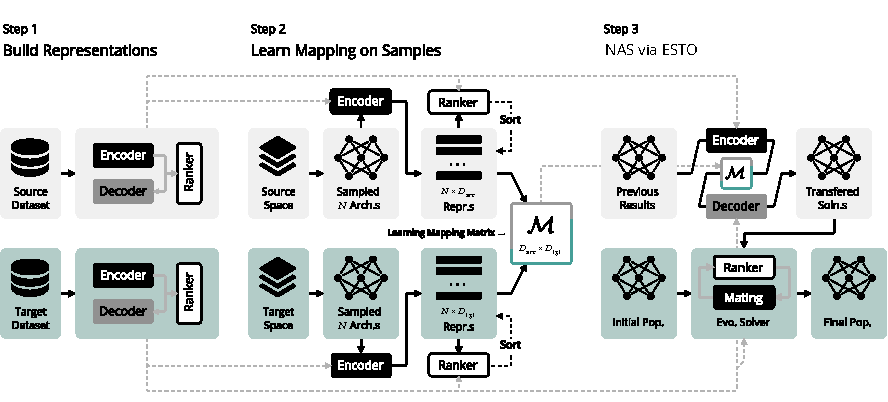
\includegraphics[width=\textwidth]{BRIDGE/overview-fixed.pdf}
	\bicaption[\textsc{Bridge}框架概览]{
		\textsc{Bridge} 框架的整体概览。
		整个流程可分为三个关键阶段:
		(1) 通过有监督与无监督表示学习构建神经架构的紧凑且语义丰富的隐式表示;
		(2) 在源域与目标域的表示空间之间学习一个结构保持的映射函数,以对齐不同搜索空间下的架构语义;
		(3) 利用所学表示模型与跨域映射,将源域中历史搜索获得的高性能架构解高效迁移至目标域,作为进化搜索的高质量初始种群,从而显著加速目标域的神经架构搜索过程。
	}[Overview of \textsc{Bridge}]{
		Overview of the \textsc{Bridge} framework.
		The workflow is divided into three key stages:
		(1) constructing compact and semantically rich latent representations of neural architectures via supervised and unsupervised representation learning;
		(2) learning a structure-preserving mapping between the source and target representation spaces to align architecture semantics across heterogeneous search spaces;
		(3) leveraging the learned representation model and cross-domain mapping to transfer high-performing source architectures into the target domain as a high-quality initial population for evolutionary search, thereby markedly accelerating target-domain NAS.
	}\label{fig:overview}
\end{figure}

本节全面阐述我们提出的跨域进化迁移神经架构搜索框架——\textsc{Bridge}~(\textbf{B}uilding \textbf{R}epresentation for \textbf{I}nter-\textbf{D}omain Hetero\textbf{g}eneous \textbf{E}volutionary TNAS)。
该框架旨在解决一个核心挑战:如何在异构搜索空间之间实现高效的知识迁移,从而避免在新任务或新硬件平台上从零开始执行昂贵的 NAS 过程。
为此,\textsc{Bridge} 并非直接迁移原始架构结构,而是通过学习架构的语义表示,并在表示空间中建立跨域映射,实现语义对齐而非结构复制的迁移范式。

我们首先对整体框架进行宏观概述,随后逐层深入剖析其三大核心组件:
(1)神经架构表示的构建——通过定制化分词器与基于 Transformer 的变分自编码器,将图结构的神经架构编码为连续、结构感知且性能可预测的隐向量;
(2)跨域表示映射的构造——在源域与目标域的表示空间之间学习一个可微或可优化的映射函数,使得源域中的高性能架构在目标域中具有语义等价的对应;
(3)基于跨域顺序迁移的进化 TNAS——将迁移后的架构作为初始种群,引导目标域上的进化搜索过程,兼顾探索与利用,有效规避负迁移风险。

这些组件协同工作,共同构成了一个通用、可扩展且任务自适应的迁移神经架构搜索(Transferable Neural Architecture Search, TNAS)系统。

如图~\ref{fig:overview} 所示,\textsc{Bridge} 的工作流程遵循“表示—映射—迁移—搜索”的四步范式。
首先,在表示学习阶段,我们分别在源域 $\mathcal{S}$ 与目标域 $\mathcal{T}$ 上独立训练神经架构表示学习器。
该学习器包含编码器、解码器与性能预测器三个模块,其目标是建立从离散架构空间到连续表示空间的双向映射,并确保该表示空间与架构性能高度相关。
值得注意的是,这一阶段无需跨域对齐,仅需各自域内的架构样本(无论是否带有性能标签),因此具有极强的部署灵活性。

随后,在映射学习阶段,我们利用少量在目标域上评估过的架构样本(通常仅需数百个),结合源域中已知的高性能架构,构建一个从源域表示空间 $\mathbb{R}_{\mathcal{S}}$ 到目标域表示空间 $\mathbb{R}_{\mathcal{T}}$ 的映射函数 $\mathcal{M}$。
该映射的关键在于:它并非简单地对齐任意架构,而是对齐性能排序相近的架构。
为此,我们采用基于性能排序的采样策略,确保映射学习聚焦于高价值区域,从而提升迁移质量。

最终,在迁移与搜索阶段,我们将源域历史搜索中获得的精英架构集合 $P_{\mathrm{src}}$ 依次编码、映射、解码,生成目标域中的初始种群 $P_0$。
该种群作为进化算法的起点,显著缩小了目标域的搜索空间,使搜索过程能够快速收敛至高性能区域。
整个框架的设计哲学在于:不依赖源域与目标域结构相似性,而是通过语义表示实现跨域知识的解耦与重用。

\mysection{统一架构编码与架构表征学习}\label{sec:ch4-5-unified-encoding-and-representation-learning}

\mysubsection{神经架构分词器}
\label{sec:ch4-5-1-nas-tokenizer}

神经架构本质上是计算图,其中数据通过图中的算子进行变换,并遵循图的流向与其他数据流交互或传递至后续算子。
因此,神经架构可自然地视为一种图结构数据,具体而言是有向无环图。
为减少信息损失,特别是配合基于 Transformer 的表示学习器,
我们引入一种神经架构分词器,将神经架构的拓扑结构与算子信息编码为序列。

为适配多种异构搜索空间,我们针对两种主流的基于单元的神经架构编码范式——节点上算子(Operation On Node, OON)与边上算子(Operation On Edge, OOE)——进行了专门设计。
该定制化策略确保分词器能够有效捕捉并表示不同神经架构的复杂特性。

\textbf{OON 编码。}
在节点上算子编码范式中(如 NASNet~\cite{learningtransferablearchitectures_zoph_2018} 与 NAS-Bench-101~\cite{nasbench101_ying_2019} 所示),
算子被视为节点,数据流被视为边。
该编码方式将拓扑信息与算子信息分别表示为邻接矩阵与节点标签。
形式化地,对于一个包含 $ n $ 个节点、采用 OON 编码的神经架构单元 $ \bm{x}=(A,\bm{ops}) $,
其中 $ A $ 为邻接矩阵,$ \bm{ops} $ 为操作符标记序列,
所提出的神经架构分词器将其编码为长度为 $ l^{\mathstrut}_\mathrm{N}+2 $ 的序列 $ \mathrm{Tkn}^{\mathstrut}_\mathrm{N}(\bm{x}) $:
\begin{empheq}[left=\empheqlbrace]{equation}
	\begin{aligned}
		 & \mathrm{Tkn}^{\mathstrut}_\mathrm{N} (\bm{x}) = \{\mathtt{CLS}\}\,\cup\, \underbracket[.5pt]{\mathrm{Triu}(A)\,\cup\,\bm{ops}_{2:n-1}}_\text{\( l^{\mathstrut}_\mathrm{N} \) tokens}\,\cup\,\{\mathtt{END}\} \\
		 & l^{\mathstrut}_\mathrm{N} = \frac{n (n-1)}{2} + (n-2) = \frac{1}{2} (n^2 + n-4)
	\end{aligned}\label{eq:oon-tokenizer}
\end{empheq}
其中,我们使用特殊标记 \texttt{CLS} 与 \texttt{END} 分别表示序列的起始与结束。
$ \mathrm{Triu}(\cdot) $ 表示给定邻接矩阵的上三角部分。
如图~\ref{fig:nb101-encoding} 所示,该编码方案包含两部分:
第一部分由 $ n(n-1)/2 $ 个标记组成,对应邻接矩阵上三角部分的展平;
第二部分由 $ n-2 $ 个标记组成,表示除输入/输出节点外的节点标签。
这些算子标签根据预定义的词汇表(见图~\ref{fig:vocabulary})映射为对应标记。

\begin{figure}[t]
	\centering
	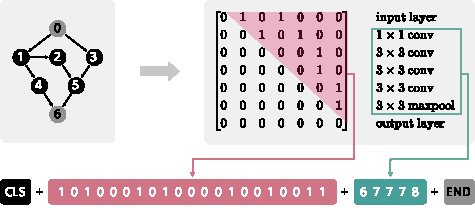
\includegraphics[width=.67\linewidth]{BRIDGE/nb101-encoding.pdf}
	\bicaption[NAS-Bench-101 OON 分词示意]{将 OON 架构(来自 NAS-Bench-101)分词为序列的示意图。
		符号 “+” 表示两个序列的拼接。}[Tokenizing an OON architecture]{Illustration of tokenizing an OON architecture from NAS-Bench-101 into a sequence. The symbol “+” denotes the concatenation of two sequences.}\label{fig:nb101-encoding}
\end{figure}

\begin{figure}
	\centering
	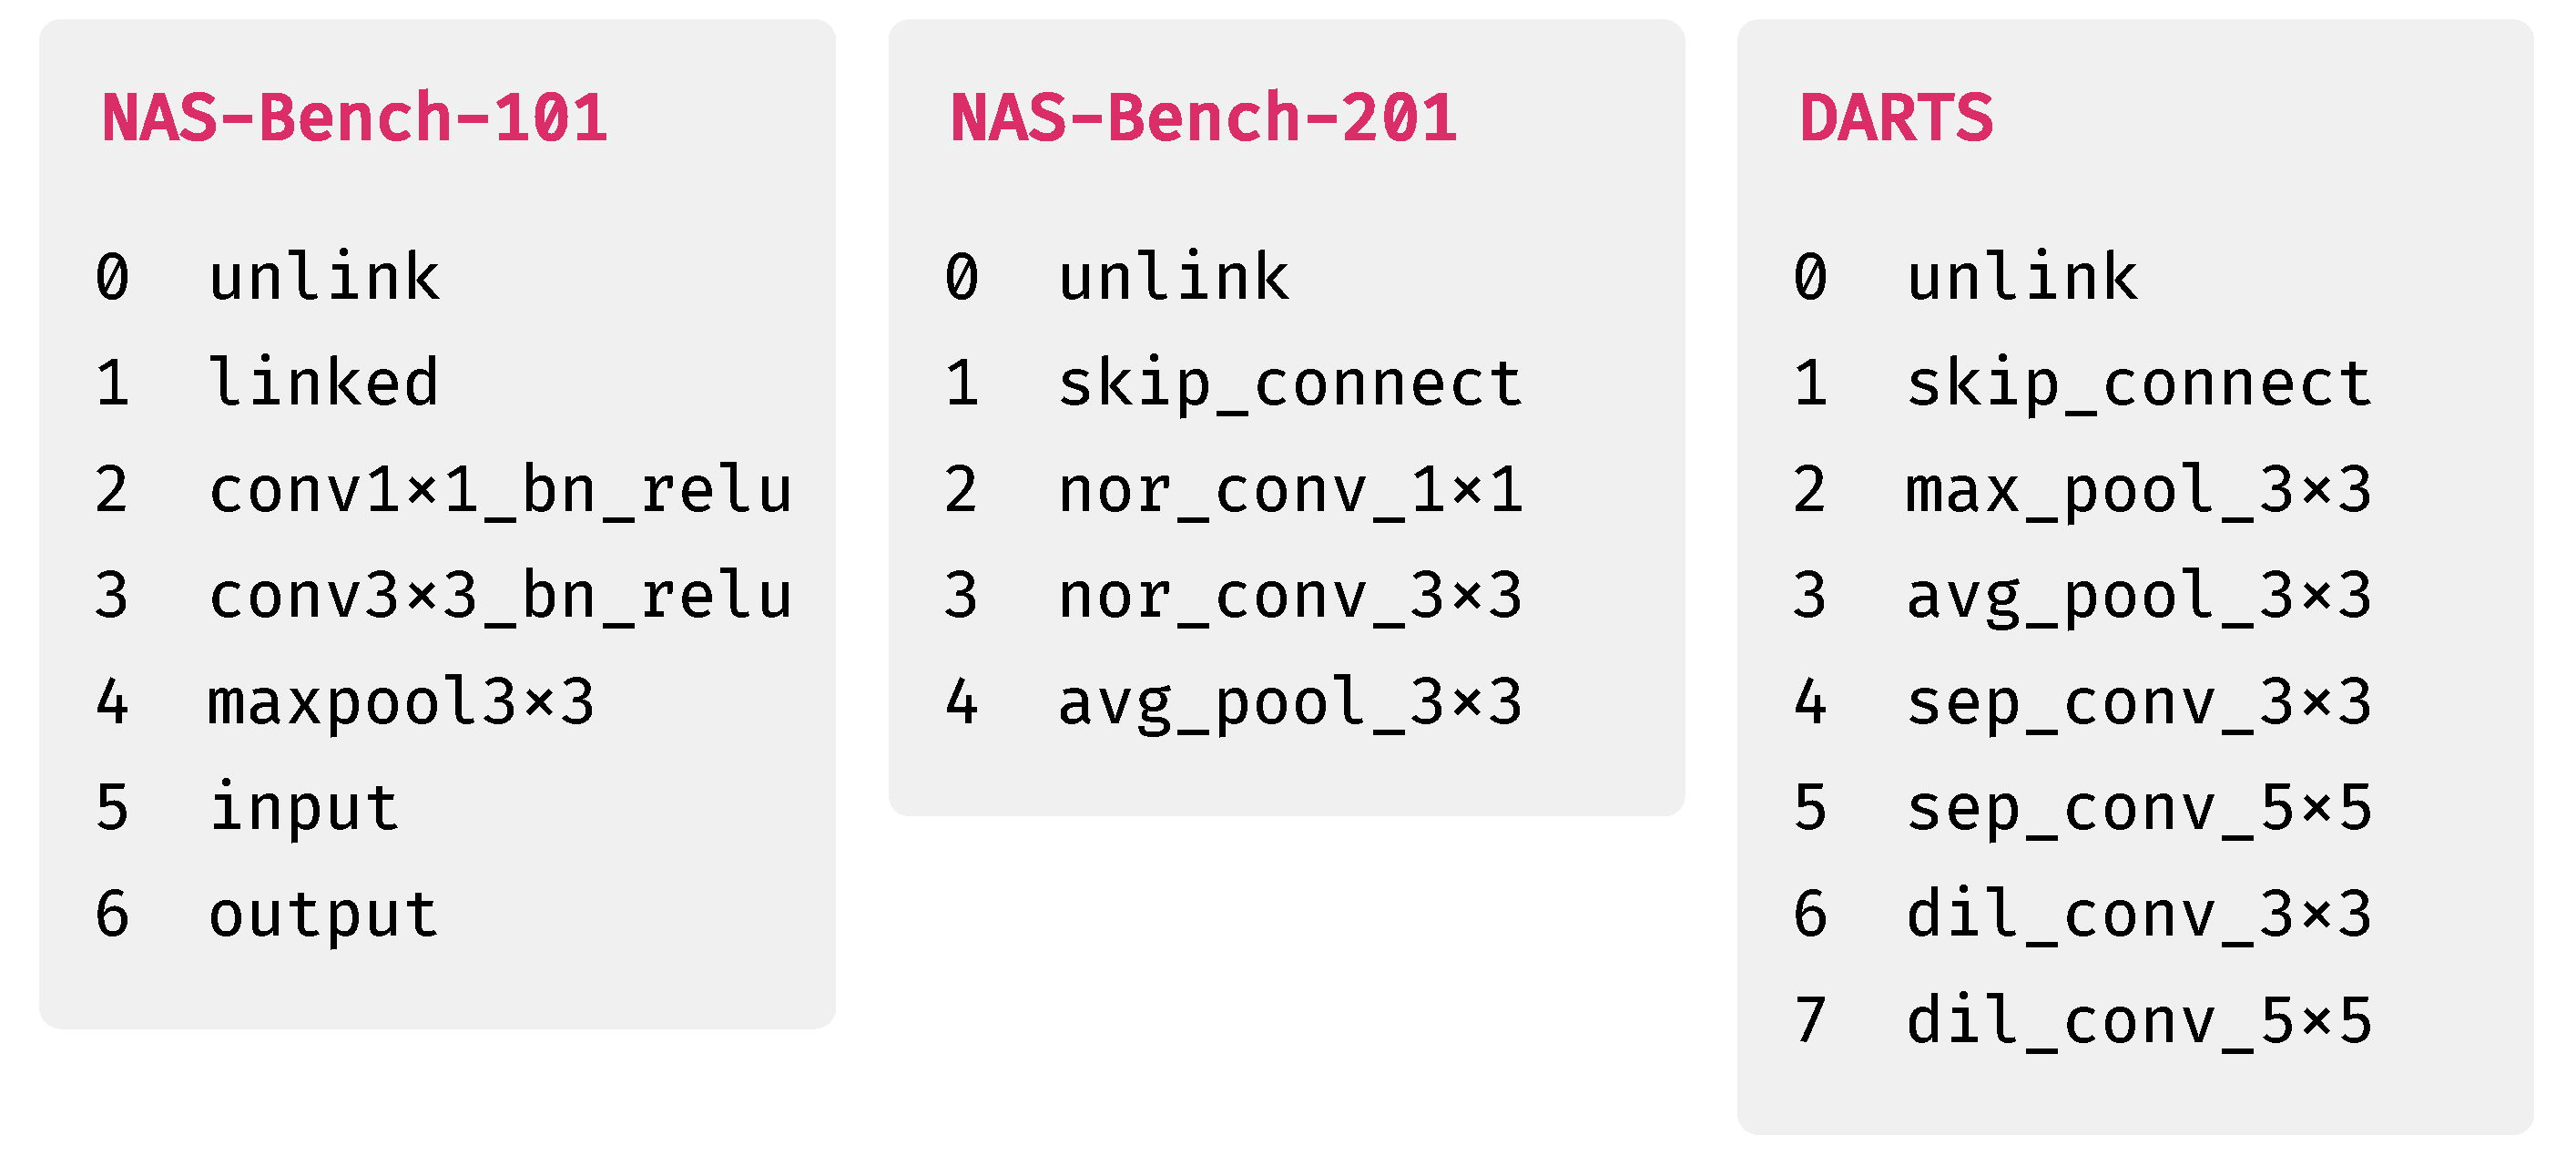
\includegraphics[width=.67\linewidth]{BRIDGE/vocabulary.pdf}
	\bicaption[算子词汇表对比]{
		NAS-Bench-101、NAS-Bench-201 与 DARTS 搜索空间各自的算子词汇表。
	}[Operator vocabularies]{
		Operator vocabularies of the NAS-Bench-101, NAS-Bench-201, and DARTS search spaces.
	}\label{fig:vocabulary}
\end{figure}

\textbf{OOE 编码。}
与 OON 编码不同,边上算子编码范式将算子视为边、数据视为节点。
该编码方式(如 DARTS~\cite{dartsdifferentiablearchitecture_liu_2019} 与 NAS-Bench-201~\cite{natsbenchbenchmarking_dong_2022} 所示)
将神经架构的拓扑与算子信息压缩至邻接矩阵中,从而实现更密集的信息表示,
更清晰地刻画算子间及其与数据节点的交互关系。
一个包含 $ n $ 个节点的神经架构单元 $ \bm{x}=(A) $ 将被编码为长度为 $ l_\mathrm{E}+2 $ 的序列 $ \mathrm{Tkn}_\mathrm{E}(\bm{x}) $:
\begin{empheq}[left=\empheqlbrace]{equation}
	\begin{aligned}
		 & \mathrm{Tkn}^{\mathstrut}_\mathrm{E} (\bm{x}) = \{\mathtt{CLS}\}\,\cup\,\underbracket[.5pt]{\mathrm{Triu} (A)}_\text{\( l^{\mathstrut}_\mathrm{E} \) tokens}\,\cup\,\{\mathtt{END}\} \\
		 & l^{\mathstrut}_\mathrm{E} = \frac{n (n-1)}{2} = \frac{1}{2} (n^2-n)
	\end{aligned}
	\label{eq:ooe-tokenizer}
\end{empheq}
其中,序列通过展平邻接矩阵的上三角部分并加入特殊标记构建而成。
特别地,当神经架构中存在多种单元类型时(例如 DARTS 搜索空间),
其对应序列将被无缝拼接,从而在统一序列表示中完整保留各类单元的独特特性。

\begin{figure*}[t]
	\centering
	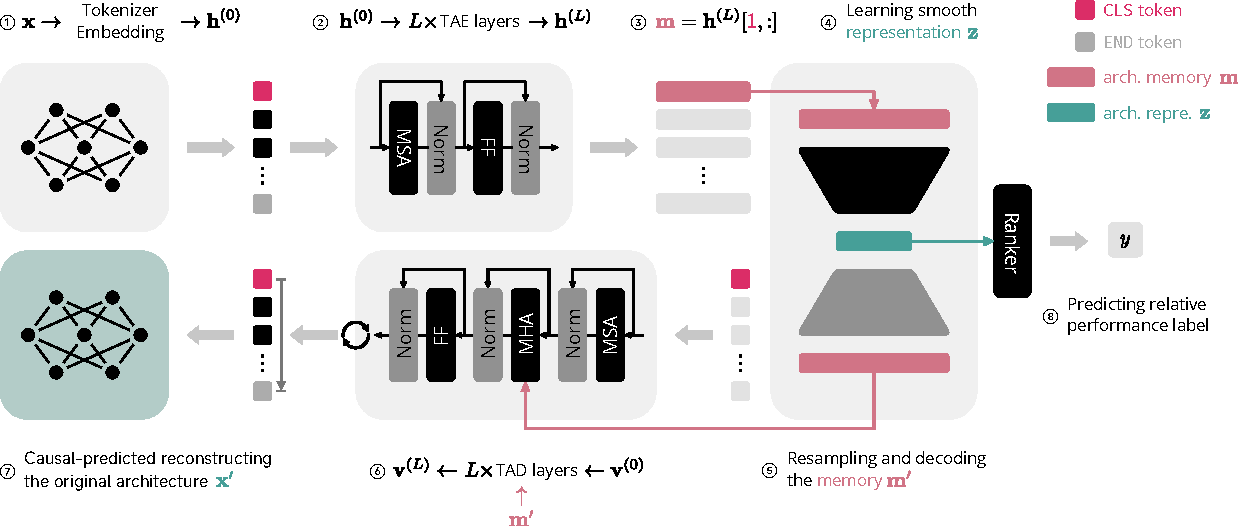
\includegraphics[width=\linewidth]{BRIDGE/repr-learner.pdf}
	\bicaption[表示学习器示意图]{
		所提表示学习器的示意图。
		在预训练阶段,仅优化神经架构重建损失,性能相对预测器不参与训练;
		在微调阶段,重建损失与预测损失联合优化。
	}[Representation learner diagram]{
		Diagram of the proposed representation learner.
		During pre-training only the neural architecture reconstruction loss is optimized and the relative performance predictor is not trained;
		during fine-tuning, the reconstruction and prediction losses are optimized jointly.
	}\label{fig:repr-learner}
\end{figure*}

\mysubsection{基于 Transformer 的变分自编码器}
\label{sec:ch4-5-2-transformer-based-variational-autoencoder}

鉴于神经架构兼具结构与语义信息的复杂特性,
我们采用 Transformer~\cite{attentionisall_vaswani_2017,narformerneural_yi_2023} 构建其表示模型。
Transformer 在处理可变长度序列方面的优势,使其特别适合编码 NAS 中遇到的多样化架构。
此外,Transformer 能够捕获输入序列中的全局交互,从而全面理解架构整体,
这对于解析架构组件间的复杂关系至关重要。
因此,Transformer 成为我们神经架构表示的理想选择,
为有效捕捉架构复杂性提供了鲁棒性、高效性与可扩展性。

表示学习器的设计基于变分自编码器框架(见图~\ref{fig:repr-learner}),
受该领域先驱工作~\cite{doesunsupervisedarchitecture_yan_2020,smoothvariationalgraph_lukasik_2021} 启发,
实现架构空间与表示空间之间的双向映射。
选择 VAE 主要基于以下优势:
首先,其单射编码特性确保局部结构信息的唯一捕获,
从而为每个架构生成唯一表示并保留丰富的结构细节;
其次,VAE 促使相似架构在隐空间中聚类,
有利于实现平滑的架构过渡。
这种平滑的隐空间对下游任务(如神经架构评估)大有裨益,
因为相似架构通常具有相近的性能~\cite{surveyevolutionaryneural_liu_2020}。
因此,神经架构表示充分利用 VAE 的上述特性,
全面理解不同架构间的复杂结构关系。

首先,参数为 $ \phi $ 的 VAE 编码器 $ q_{\phi}(\bm{z}|\bm{x}) $ 将输入数据 $ \bm{x} $
(即从未知分布中独立同分布采样的有限样本)映射为连续隐变量 $ \bm{z} $。
随后,称为解码器的概率生成模型 $ p_{\theta}(\bm{x}|\bm{z}) $ 将隐变量 $ \bm{z} $ 重构回原始表示。
编码器与解码器的参数 $ \phi $ 与 $ \theta $ 通过最大化下式进行优化:
\begin{equation}\label{eq:vae-loss}
	\mathcal{L}_{\phi,\theta}{(\bm{x})} = \underbrace{\mathbb{E}_{\bm{z} \sim q_{\phi}(\bm{z}|\bm{x})}{\big[\log{p_\theta(\bm{x}|\bm{z})}\big]}}_{\text{重建损失}} \:{-}\: \underbrace{D_\mathrm{KL}\big(q_\phi(\bm{z}|\bm{x})\:\|\:p_\theta(\bm{z})\big)}_{\text{正则化项}}
\end{equation}
其中第一项为证据下界,即重建损失,
确保输入数据与解码器生成数据的高度相似性,在保持原始与重构数据保真度方面起关键作用;
第二项为Kullback-Leibler 散度,作为隐空间的正则项,
促使隐变量分布接近先验分布,从而构建结构良好、行为规范的隐空间。

以下详述所设计的基于 Transformer 的 VAE 编码器与解码器,
以有效捕获并重构神经架构中的复杂结构关系。

\mysubsubsection{神经架构编码器}

对于给定神经架构 $ \bm{x} $,在输入 Transformer 编码器前需进行若干变换。
首先,使用式~(\ref{eq:oon-tokenizer}) 或式~(\ref{eq:ooe-tokenizer}) 将其分词为离散标记序列,
每个标记代表特定架构组件或操作,以确保与 Transformer 编码器格式兼容。
随后,每个标记通过可学习嵌入层 $ \mathrm{Emd}(\cdot) $ 映射为高维嵌入向量,
以捕获架构组件间的语义关系。
接着加入位置嵌入 $ E_\mathrm{pos} $,为 Transformer 编码器提供顺序信息,
如式~(\ref{eq:enc-embedding}) 所示。

所得嵌入序列(含位置信息)输入 Transformer 编码器,
经多头自注意力层 $ \mathrm{MSA}(\cdot) $ 与前馈层 $ \mathrm{FF}(\cdot) $ 处理,
生成神经架构的上下文表示。
每层输入应用层归一化 $ \mathrm{LN}(\cdot) $,并加入残差连接,
遵循典型 Transformer 层设计。
形式化地,架构 $ \bm{x} $ 可通过 $ N $ 层基于 Transformer 的架构编码器 $ \mathrm{TAE}(\cdot) $ 编码为:
\begin{empheq}[
		left={\mathrm{TAE}(\bm{x})\Rightarrow \empheqlbrace}
	]{alignat=2}
	& \bm{h}^{(0)} & = {} & \mathrm{Emd} (\mathrm{Tkn} (\bm{x})) + E_\mathrm{pos}\label{eq:enc-embedding}          \\
	& \bm{h}_\mathrm{att}^{(i)} & = {} & \mathrm{LN} (\mathrm{MSA} (\bm{h}^{(i-1)})) + \bm{h}^{(i-1)}                \notag{} \\
	& \bm{h}^{(i)} & = {} & \mathrm{LN} (\mathrm{FF} (\bm{h}_\mathrm{att}^{(i)})) + \bm{h}_\mathrm{att}^{(i)}                     \notag{}
\end{empheq}
其中 $ i \in [1,N] $,$ \bm{h}^{(i)} $ 与 $ \bm{h}_\mathrm{att}^{(i)} $ 分别表示第 $ i $ 层的隐藏状态与注意力状态。

特别地,\texttt{CLS} 标记的隐藏状态被用作输入架构序列的记忆,
由此可计算两个表示:
\begin{align}
	\bm{m}          & = \bm{h}^{(N)}[1,:]            \\
	\bm{r}_{\mu}    & = \mathrm{FC}_{\mu}(\bm{m})    \\
	\bm{r}_{\sigma} & = \mathrm{FC}_{\sigma}(\bm{m})
\end{align}
其中 $ \bm{m} $ 表示输入架构的记忆,
$ \bm{r}_{\mu} $ 与 $ \bm{r}_{\sigma} $ 分别为所学神经架构表示分布的均值与方差。
两个 $ \mathrm{FC}(\cdot) $ 为相同设置的全连接层。
因此,编码器输出为近似后验分布的参数:
\begin{equation}
	q_\phi(\bm{z}|\bm{x}) = \mathcal{N}(\bm{z};\bm{r}_\mu,\varSigma),
\end{equation}
其中 $ \varSigma = \bm{r}_{\sigma}I $ 为多元正态分布的协方差矩阵。

\mysubsubsection{神经架构解码器}

基于 Transformer 的 VAE 解码器 $ p_{\theta}(\bm{x}|\bm{z}) $ 以隐变量点 $ \bm{z} $ 为输入,
重构 $ \bm{x} $。
为确保最优重建稳定性,原始架构 $ \bm{x} $(长度可变)基于重构记忆以因果预测方式重建(见算法~\ref{algm:causal-predict})。
通过带激活函数的线性层,获得重构记忆 $ \bm{m}^\prime = \mathrm{ReLU}(\mathrm{FC}(\bm{z})) $。
重建过程从仅含 \texttt{CLS} 的初始序列开始,
递归预测下一标记,直至遇到 \texttt{END} 标记或序列达到最大长度 $ L $。
\begin{equation}
	\mathrm{TAD}(\bm{y};\bm{m}^\prime)\Rightarrow\left\{
	\begin{alignedat}{2}
		 & \bm{v}^{(0)} & = {} & \mathrm{Emd} (\mathrm{Tkn} (\bm{y})) + E_\mathrm{pos}                   \\
		 & \bm{s}^{(i)} & = {} & \mathrm{LN} (\mathrm{MSA} (\bm{v}^{(i-1)})) + \bm{v}^{(i-1)}            \\
		 & \bm{c}^{(i)} & = {} & \mathrm{LN} (\mathrm{MHA} (\bm{m}^\prime, \bm{s}^{(i)})) + \bm{s}^{(i)} \\
		 & \bm{v}^{(i)} & = {} & \mathrm{LN} (\mathrm{FF} (\bm{c}^{(i)})) + \bm{c}^{(i)}
	\end{alignedat}\right.
\end{equation}
其中 $ i \in [1,N] $,$ \bm{v}^{(i)} $ 表示解码器第 $ i $ 层的隐藏状态,
$ \bm{s}^{(i)} $ 与 $ \bm{c}^{(i)} $ 分别表示多头自注意力的中间状态。

\begin{algorithm}[t]
	\caption{架构因果重建}\label{algm:causal-predict}
	\SetAlgoLined{}
	\KwIn{编码器记忆 $ \mathbf{m^\prime} $,初始标记 $ y_0 $}
	\KwOut{完整输出序列 $ \bm{y} $}
	\BlankLine
	初始化 $ \bm{y} \gets \{y_0\} $\;
	\BlankLine
	\For{\( t \gets 1 \) \KwTo \( T \)}{
		解码器隐藏状态 $ \bm{v}_{t} \gets \mathrm{TAD}(\bm{y}) $\;
		计算标记概率分布 $ p(y_{t}|\mathbf{h}) $\;
		从 $ p(y_t|\bm{h}) $ 中采样标记 $ y_t $\;
		将 $ y_t $ 追加至 $ \bm{y} $\;
		\lIf{\( y_t = \mathtt{END} \)}{break}
	}
	\BlankLine
	\Return{\( \bm{y} \)}\;
\end{algorithm}

\mysubsection{神经架构相对性能预测器}
\label{sec:ch4-5-3-nas-relative-performance-predictor}

此处的主要目标是利用架构的性能度量建立不同搜索空间对应表示空间之间的映射,
从而促进跨域解的迁移,提升搜索效率与效果。
为增强神经架构表示的学习过程,我们提出引入与架构性能相关的有监督信号。
具体而言,我们采用神经架构性能预测器快速评估架构或其表示。
该预测器用于调整架构表示的分布,使其更聚焦于性能指标。
此外,预测器还用于构建表示空间间的映射,
通过高效提供期望的性能标签,使模型更好地理解架构表示与其性能之间的关系,
从而引导搜索过程朝向高性能解。

受到 ReNAS~\cite{renasrelativisticevaluation_xu_2021} 设计的启发,
我们引入一个神经架构相对性能预测器(即排序器),
由带激活函数的多层感知机构成。
鉴于 NAS 的评估策略主要关注发现更优架构而非单个架构的具体性能,
放松性能预测目标是有益的。
通过聚焦于捕获架构性能的相对差异,模型能更有效地区分架构排名。
给定一组架构表示 $ Z = {\{ \bm{z}^{i} \}}_{1}^{n} $,
该相对预测器可通过优化下式进行训练:
\begin{gather}
	\begin{aligned}
		\Delta_{\mathrlap{\mathrm{pred}}}^{(i,j)}(Z) & = \psi_{\omega}(\bm{z}^i) - \psi_{\omega}(\bm{z}^j) \\
		\Delta_{\mathrlap{\mathrm{sign}}}^{(i,j)}(Z) & = \mathrm{Sign}(y_i-y_j)
	\end{aligned} \notag \\
	\mathcal{L}_\mathrm{rel} = \sum_{\mathclap{i=1}}^{n-1}{\;\sum_{\mathclap{j=i+1}}^{n}{\exp{\left( \Delta_\mathrm{pred}^{(i,j)}(Z) \times \Delta_\mathrm{sign}^{(i,j)}(Z)\right)}}}
\end{gather}
其中 $ \psi_\omega(\cdot) $ 为性能预测器输出,
$ \Delta_{\mathrm{pred}}^{(i,j)}(Z) $ 表示预测性能差异,
$ \Delta_{\mathrm{sign}}^{(i,j)}(Z) $ 衡量真实性能的相对排序。

\mysubsection{混合监督训练}
\label{sec:ch4-5-4-mixed-supervision-training}

神经架构表示的构建包含无监督预训练与有监督微调两个阶段,
二者目标不同但互补,共同实现鲁棒且可迁移的表示。

在预训练阶段,表示学习器通过编码与解码处理源域与目标域的神经架构,
建立对架构模式与特征的基础理解,且不依赖性能指标。
随后的微调阶段则引入任务特定的性能数据,
在保持可迁移性的同时优化目标域表示。
该监督阶段校准所学表示,使其与领域特定需求及性能目标对齐。

该双阶段方法最小化对标记数据的依赖,
在性能测量有限的新领域尤为宝贵。
无监督预训练实现对架构模式的广泛识别,
而微调确保领域特定优化。
总体而言,该方法在知识迁移与领域适应之间取得平衡,
实现高效跨域知识迁移,同时不损害表示质量或任务相关性。

\mysubsubsection{无监督预训练:神经架构重建}

神经架构表征学习器需要对架构的结构与语义信息进行深入理解,这需要大量数据作为支撑。
预训练阶段利用大量未标记数据驱动无监督学习,
避免获取神经架构性能标签的高昂成本。
此阶段优化目标主要围绕最小化重建损失,
模型力求从表示空间忠实地重构架构配置。
基于式~(\ref{eq:vae-loss}),重建损失与正则化损失可描述为:
\begin{align}
	\mathcal{L}_\mathrm{rec} & = \mathbb{E}_{\bm{z} \sim q_{\phi}(\bm{z}|\bm{x})}{\big[\log{p_\theta(\bm{x}|\bm{z})}\big]}                                   \\
	\mathcal{L}_\mathrm{reg} & = {-}D^{\mathstrut}_\mathrm{KL}\big(q_\phi(\bm{z}|\bm{x})\:\|\:p_\theta(\bm{z})\big) \notag                                   \\
	{}                       & = {-}\frac{1}{2}\sum{\left({1+\log{(\bm{r}^{\mathstrut}_{\sigma}) - \bm{r}_{\mu}^{2} - \bm{r}^{\mathstrut}_{\sigma}}}\right)}
\end{align}

在框架的预训练阶段,一个显著特点是相对性能预测器(排序器)刻意保持不活跃。
该组件在此阶段不参与训练。
我们采用优化目标解耦策略,
使模型学习不依赖领域特定性能指标的通用架构特征。
该解耦过程有助于捕获内在架构特性,
促进更通用且可迁移的表示构建,
为后续跨域迁移任务奠定坚实基础。
形式化地,优化目标可表示为:
\begin{equation}
	\mathcal{L}_\mathrm{pt} = \mathcal{L}_\mathrm{rec} + \alpha\mathcal{L}_\mathrm{reg}
\end{equation}
其中 $ \alpha $ 为平衡重建损失与正则化损失的权重因子。

\mysubsubsection{混合监督微调:相对性能预测}

在微调阶段,神经架构表征学习器通过有监督学习技术进行精细化调整。
此阶段以稀缺但关键的标记数据为核心,提升表示映射的预测能力。
微调采用联合优化框架,使重建损失与预测损失协同优化,
引导模型生成的表示不仅捕获架构结构细节,
还能有效预测其在不同任务域中的相对性能。
该阶段最终产生精细校准的神经架构表示,
为异构环境中的无缝知识迁移与领域适应做好准备。
此阶段的优化目标函数如下:
\begin{equation}
	\mathcal{L}_\mathrm{ft} = \mathcal{L}_\mathrm{rec} + \alpha\mathcal{L}_\mathrm{reg} + \beta\mathcal{L}_\mathrm{rel}
\end{equation}
其中 $ \mathcal{L}_\mathrm{rel} $ 为相对性能预测损失,
超参数 $ \alpha $ 与 $ \beta $ 控制各组件间的平衡,
实现对学习过程的精细调控。

\mysection{构建跨域表征映射}
\label{sec:ch4-6-building-cross-domain-embeddings}

基于前述架构表示学习器的组件,NAS 解可通过所提 \textsc{Bridge} 显式迁移至其他领域的任务。
如图~\ref{fig:overview} 所示,以下步骤聚焦于构建源域与目标域表示空间之间的映射,
实现神经架构解的显式跨域迁移。
通过建立该映射,模型可有效利用源域知识提升目标域的搜索效率,发现高性能架构。

构建源域与目标域表示空间间的映射对跨域知识迁移至关重要。
令 $ \mathbb{R}^{\mathstrut}_{\mathcal{S}} $ 与 $ \mathbb{R}^{\mathstrut}_{\mathcal{T}} $ 分别表示源域($ \mathcal{S} $)与目标域($ \mathcal{T} $)的表示空间。
目标是学习映射函数 $ \mathcal{M}: \mathbb{R}^{\mathstrut}_{\mathcal{S}} \rightarrow \mathbb{R}^{\mathstrut}_\mathcal{T} $,
最小化源域映射表示与目标域对应表示间的差异。
形式化地,待最小化的目标函数为:
\begin{equation}
	\mathcal{L}_\mathrm{map}(\mathcal{M}) = \sum_{i=1}^{N}{\ell\left(\mathcal{M}(\bm{z}_{s}^{(i)}),\bm{z}_{t}^{(i)}\right)}
\end{equation}
其中 $ \bm{z}^{(i)}_{s} \in \mathbb{R}^{\mathstrut}_{\mathcal{S}} $ 与 $ \bm{z}^{(i)}_{t} \in \mathbb{R}^{\mathstrut}_{\mathcal{T}} $ 分别为按预测值排序后第 $ i $ 个采样表示,
$ N $ 为采样表示对总数,$ \ell $ 为衡量映射源表示与目标表示差异的损失函数。
映射函数 $ \mathcal{M} $ 的选择取决于表示空间特性及所需灵活性与复杂度。
本文以线性映射为例:$ \mathcal{M}(\bm{z}_{s}) = \bm{z}_{s}W + \bm{b} $,
其中 $ W $ 与 $ \bm{b} $ 为可学习的权重矩阵与偏置向量。
采用均方误差作为 $ \ell $,映射通过优化下式学习将源域表示投影至目标域:
\begin{equation}
	\min_{W,\mathbf{b}} \mathcal{L}_\mathrm{map}(\mathcal{M}) = \frac{1}{N}\sum_{i=1}^{N}{\left\|\bm{z}_{t}^{(i)} - \left(\bm{z}_{s}^{(i)}W + \bm{b}\right)\right\|}^{2}.
\end{equation}

\mysection{跨空间演化贯序迁移的神经架构搜索}
\label{sec:ch4-7-progressive-transfer-nas-across-spaces}

基于所构建的跨域神经架构映射,我们进一步设计了 ESTO 算法——
一种基于种群的方法,能高效实现域间解的显式迁移。

我们的迁移方法与求解器在设计上解耦,允许使用多种求解器。
然而,我们选择进化求解器因其独特优势:
首先,进化算法天然维持多样化解集,可在整合迁移架构的同时保持探索能力,
这种基于种群的方法比单解方法提供更鲁棒的知识迁移;
其次,进化交叉操作为结合迁移知识与新颖架构模式提供了有效机制,
使搜索过程既能利用先验经验,又能发现针对目标域定制的新解;
此外,进化方法对架构表示施加的约束更少,
特别适合源域与目标域搜索空间存在差异的跨域迁移场景。

该方法利用源域的最优神经架构种群初始化并引导目标域的进化搜索过程,
高效探索目标搜索空间中的有希望区域。
在源域中,框架首先利用预训练性能预测器识别最优神经架构种群,
选取表现最佳的个体形成精英种群,体现源域积累的知识。
\textsc{Bridge} 中所提 ESTO 算法概览见算法~\ref{algm:ch4-transfer},流程如下:
\begin{itemize}[leftmargin=3\ccwd]
	\item \textbf{知识编码(第 1–2 行):} 从源域最优种群中选取的架构通过源域编码器编码为表示向量,捕获源域中发现的高性能架构本质。
	\item \textbf{跨域映射(第 3 行):} 为将知识迁移至目标域,编码表示通过所学映射函数 $ \mathcal{M} $ 从源域表示空间映射至目标域表示空间,有效将源域最优解投影至目标域架构搜索空间。
	\item \textbf{初始种群播种(第 4–6 行):} 目标域中的映射表示作为进化搜索的初始种群,该种群以迁移知识为种子,为目标域架构搜索空间探索提供战略性起点。
	\item \textbf{进化搜索(第 7–12 行):} ESTO 过程随后以常规进化算法进行,但关键区别在于搜索过程受源域迁移知识引导。
	      在目标域上训练的性能预测器 $ \mathrm{Rkr}^{\mathstrut}_{\mathcal{T}}(\cdot) $ 用于评估新架构的适应度,确保搜索针对目标域特性进行定制。
\end{itemize}

\begin{algorithm}[t!]
	\SetAlgoLined{}
	\let\oldnl\nl % Store \nl in \oldnl
	\newcommand{\nonl}{\renewcommand{\nl}{\let\nl\oldnl}}% Remove line number for one line
	\caption{\textsc{Bridge} 的所提出的 ESTO 算法}\label{algm:ch4-transfer}
	\KwIn{$P^{\mathstrut}_\mathrm{src}$,源域历史 NAS 过程获得的待迁移解集;$G$,最大进化代数。}
	\KwOut{$P^{\mathstrut}_\mathrm{rst}$,目标域上搜索得到的最终种群。}

	\BlankLine{}

	\tcc{准备工作}
	\( \big[\mathrm{Enc}^{\mathstrut}_{\mathcal{S}}(\cdot), \mathrm{Dec}^{\mathstrut}_{\mathcal{S}}(\cdot), \mathrm{Rkr^{\mathstrut}}_{\mathcal{S}}(\cdot)\big] \gets \) 在源域上学习表征;

	\( \big[\mathrm{Enc}^{\mathstrut}_{\mathcal{T}}(\cdot), \mathrm{Dec}^{\mathstrut}_{\mathcal{T}}(\cdot), \mathrm{Rkr}^{\mathstrut}_{\mathcal{T}}(\cdot)\big] \gets \) 在目标域上学习表征;

	\(\mathcal{M} \gets \) 学习从 \( \mathbb{R}^{\mathstrut}_{\mathcal{S}} \) 到 \( \mathbb{R}^{\mathstrut}_{\mathcal{T}} \) 的映射\;

	\BlankLine{}

	\tcc{顺序迁移}
	\( {R}^{\mathstrut}_\mathrm{src} \gets \mathrm{Enc}^{\mathstrut}_{\mathcal{S}} ({P}^{\mathstrut}_\mathrm{src}) \)\;
	\( {R}^{\mathstrut}_\mathrm{tgt} \gets \mathcal{M}({R}^{\mathstrut}_\mathrm{src}) \)\;
	\( {P}^{\mathstrut}_{0} \gets \mathrm{Dec}^{\mathstrut}_{\mathcal{T}}({R}^{\mathstrut}_\mathrm{tgt}) \)\;

	\BlankLine{}

	\tcc{进化 NAS}
	\For{\( g \) 从 \( 1 \) 到 \( G \)}{
		\( P^{\mathstrut}_\mathrm{new} \gets \) 对 \(P^{\mathstrut}_{g-1}\) 应用进化操作\;
		\( F^{\mathstrut}_\mathrm{new} \gets \mathrm{Rkr}^{\mathstrut}_{\mathcal{T}}(P^{\mathstrut}_\mathrm{new}) \)\;
		\( P^{\mathstrut}_{g} \gets \) 从 \( P^{\mathstrut}_{g} \cup P^{\mathstrut}_{\mathrm{new}} \) 中进行二元锦标赛选择\;
	}
	\( P^{\mathstrut}_\mathrm{rst} \gets P^{\mathstrut}_{g} \)\;

	\BlankLine{}

	\Return{\(P^{\mathstrut}_\mathrm{rst}\),目标域上的最终种群。}
\end{algorithm}

迁移学习中的一个关键挑战是负迁移——迁移知识与目标任务需求的根本性不匹配。
所提 \textsc{Bridge} 通过多重结构机制缓解该现象:
首先,我们的进化优化策略通过三项关键设计在整个搜索过程中保持种群多样性:
(1) 基于种群的范式即使在部分迁移解表现不佳时仍保持探索能力,可通过后续进化操作恢复;
(2) 迁移概率参数调控初始种群中迁移知识的比例,确保在利用先验知识的同时保留目标域中新解的发现能力;
(3) 自适应选择机制严格依据目标任务目标评估迁移架构,系统性地在进化周期中淘汰次优候选。

通过将进化算法与跨域迁移能力结合,\textsc{Bridge} 有效利用来自不同搜索空间的现有 NAS 解与知识,
有望在新领域中实现更高效、更有效的神经架构搜索。

\mysection{实验设置与结果分析}\label{sec:ch4-8-setup-and-results-analysis}

本节对所提出的跨域 TNAS 框架 \textsc{Bridge} 进行了全面的实验评估,以验证其有效性。我们在不同规模的搜索空间中开展了一系列实验,并对结果进行了深入分析。此外,为严格检验框架中各组成部分及设计选择的作用,我们设计了一组深入研究实验。这些研究旨在阐明我们方法中每个关键要素的贡献,并为我们的方法论决策提供实证支持。

\mysubsection{搜索空间与数据集}
\label{sec:ch4-8-1-search-space-and-datasets}

为严格评估 \textsc{Bridge},我们选取了三个神经架构搜索空间:NAS-Bench-201、NAS-Bench-101 和 DARTS。这些搜索空间在复杂度上逐级递增,为验证提供了结构化的框架。实验设计采用渐进式复杂度范式,从约束更强的搜索空间起步,逐步过渡到更复杂的领域。这种分层方法具有双重目的:一方面验证所提方法的可扩展性,另一方面系统性地探究在日益贴近现实的架构场景中知识迁移的能力。该渐进过程最终在足够复杂的搜索空间中进行评估,以应对现实世界的计算挑战。

\textbf{NAS-Bench-201 空间。}~\cite{natsbenchbenchmarking_dong_2022}
该空间采用边操作(Operator-on-Edge, OOE)方案,将架构表示为有向无环图。图中每条边对应一种操作,如 \texttt{NONE}、\texttt{SKIP-CONNECT}、\texttt{CONV-1X1}、\texttt{CONV-3X3} 或 \texttt{AVG-POOL-3X3}。该空间共包含 15,625 种唯一架构,是评估 NAS 方法的有效起点。

\textbf{NAS-Bench-101 空间。}~\cite{nasbench101_ying_2019}
复杂度进一步提升,NAS-Bench-101 采用基于单元的 DAG 架构,使用节点操作(Operator-on-Node, OON)方案。节点对应 \texttt{CONV-3X3}、\texttt{CONV-1X1} 和 \texttt{MAX-POOL-3X3} 等操作,张量边连接各节点。搜索空间包含最多 7 个算子和 9 条连接的架构,总计 423,624 种唯一配置。该空间对 NAS 算法提出了适应性和可扩展性的挑战。

\textbf{DARTS 空间。}~\cite{dartsdifferentiablearchitecture_liu_2019}
代表更高复杂度,DARTS 将架构建模为计算单元,同样以 DAG 形式组织,但支持更多样化的操作集合。每个单元包含 7 个节点,输入张量按顺序流经这些节点。支持的操作包括 \texttt{MAX-POOL-3X3}、\texttt{AVG-POOL-3X3}、\texttt{SKIP-CONNECT}、\texttt{SEP-CONV-3X3}、\texttt{SEP-CONV-5X5}、\texttt{DIL-CONV-3X3} 和 \texttt{DIL-CONV-5X5}。DARTS 使用普通单元维持空间分辨率,使用缩减单元进行下采样。该空间包含超过 $10^{18}$ 种潜在架构组合,是评估大规模 NAS 性能的严格基准。

\begin{table}
	\centering
	\bicaption[表征学习超参数配置]{不同搜索空间上神经架构表征学习的超参数配置}[Hyperparameter settings]{Hyperparameter configurations for neural architecture representation learning across different search spaces}\label{tab:train-settings}

	\newcommand*{\sizefn}{\tabularnote{用于训练的样本数量,括号内为其占整个搜索空间的比例。其他规模同理。}}

	\small\begin{NiceTabularX}{\linewidth}{p{2cm}Xccc}[notes,tabularnote={\textit{pt} = 预训练, \textit{ft} = 微调, \textit{repr} = 表征, \textit{ff} = 前馈, \textit{enc-lyr} = 编码器层数, \textit{dec-lyr} = 解码器层数。}]
		\toprule
		&                             & \bfseries NB201 & \bfseries NB101 & \bfseries DARTS \\
		\midrule\midrule
		\Block{4-1}{\bfseries 训练设置}          & \textit{pt-size}\:\sizefn{} & 5,000~(50\%)    & 12,000~(30\%)   & 30,000~(--)     \\
		& \textit{ft-size}            & 1,000~(10\%)    & 4,000~(1\%)     & 1,500~(--)      \\
		\cmidrule{2-5}
		& \textit{pt-epoch}           & 200             & 200             & 200             \\
		& \textit{ft-epoch}           & 200             & 200             & 200             \\
		\midrule\midrule
		\Block{6-1}{\bfseries 模型设置}          & \textit{repr-dim}           & 64              & 64              & 128             \\
		& \textit{model-dim}          & 128             & 128             & 512             \\
		& \textit{ff-dim}             & 256             & 256             & 2,048           \\
		\cmidrule{2-5}
		& \textit{n-enc-lyr}          & 4               & 4               & 4               \\
		& \textit{n-dec-lyr}          & 4               & 4               & 4               \\
		& \textit{n-head}             & 4               & 4               & 4               \\
		\bottomrule
	\end{NiceTabularX}
\end{table}

\begin{table}[t]
	\centering
	\bicaption[表征方法性能对比]{神经架构表征学习方法的性能对比分析}[Representation learning comparison]{Performance comparison of neural architecture representation learning methods}\label{tab:repr-learn-metrics}
	\newcommand*{\trainfn}{\tabularnote{与其他方法不同,我们提出的方法保持编码器和解码器的灵活性,允许将性能数据融入表征学习过程。然而,这也带来了一定权衡,即重建精度略有下降。}}
	\newcommand*{\dartsfn}{\tabularnote{该结果基于我们在 DARTS 空间中收集的标签。}}
	\small\begin{NiceTabularX}{\linewidth}{p{6em}lXccc}[notes]
		\toprule
		&                                               &                                                   & \bfseries NB201 & \bfseries NB101 & \bfseries DARTS  \\
		\midrule\midrule
		\Block{5-1}{\bfseries 重建准确率 (\%)}                         & \Block{5-1}{\bfseries\scriptsize\textuparrow} & \textit{arch2vec}~\cite{doesunsupervisedarchitecture_yan_2020} & 99.99           & 98.84           & --               \\
		&                                               & SVGe~\cite{smoothvariationalgraph_lukasik_2021}         & 99.99           & 99.57           & 99.63            \\
		&                                               & DGMG~\cite{learningdeepgenerative_li_2018}     & 99.97           & 98.99           & 99.29            \\
		\cmidrule{3-6}
		&                                               & \textsc{Bridge} (Ptd.)                            & 99.99           & 99.90           & 99.25            \\
		&                                               & \textsc{Bridge} (Ftd.)                            & 99.06           & 99.99           & 99.12            \\
		\midrule\midrule
		\Block{4-1}{\bfseries 预测 Kendall's \( \bm{\tau} \)-b}        & \Block{4-1}{\bfseries\scriptsize\textuparrow} & NAO~\cite{neuralarchitectureoptimization_luo_2018}               & 0.526           & 0.775           & --               \\
		&                                               & TNASP~\cite{tnasptransformerbased_lu_2021}              & 0.724           & 0.820           & --               \\
		&                                               & ReNAS-6~\cite{renasrelativisticevaluation_xu_2021}          & --              & 0.816           & --               \\
		\cmidrule{3-6}
		&                                               & \textsc{Bridge}                                   & \textbf{0.827}  & \textbf{0.848}  & 0.811~\dartsfn{} \\
		\bottomrule
	\end{NiceTabularX}
\end{table}

\begin{sidewaystable}[htbp]
	\centering
	\renewcommand{\arraystretch}{1.3}
	\bicaption[NB101搜索结果]{NAS-Bench-101 空间上的神经架构搜索结果}[NAS-Bench-101 results]{Neural architecture search results on the NAS-Bench-101 space}\label{tab:transfer-result-101}
	\newcommand*{\ttestFn}{\tabularnote{第一部分的 p 值相对于 \textsc{Bridge} 计算,后续部分则相对于各自基线计算。p 值低于 0.05 表示我们的方法显著优于对比算法或非迁移基线。}}
	\small\begin{NiceTabularX}{\textwidth}{p{8em}*{2}{>{\centering\arraybackslash}X}*{3}{c}l}
		\toprule
		\RowStyle[nb-rows=1,bold]{}
		方法                                           & \Block{1-1}{最优准确率~(\%)} & \Block{1-1}{平均准确率~(\%)} & 评估次数 & \Block{1-1}{耗时 (秒)} & P 值~\ttestFn{}    & 方法类型             \\
		\midrule\midrule
		ENAS~\cite{efficientneuralarchitecture_pham_2018}                & 92.54                        & 91.83\(\,\pm\,\)0.42         & --         & --                     & 6.52E-08           & 强化学习             \\
		FBNet~\cite{fbnethardwareaware_wu_2019}      & 93.98                        & 92.29\(\,\pm\,\)1.25         & --         & --                     & 2.01E-03           & 基于梯度             \\
		CTNAS~\cite{contrastiveneuralarchitecture_chen_2021}       & 94.14                        & 93.93\(\,\pm\,\)0.12         & --         & --                     & 2.08E-01           & 预测器               \\
		ReNAS~\cite{renasrelativisticevaluation_xu_2021}         & 94.07                        & 93.95\(\,\pm\,\)0.09         & --         & --                     & 3.08E-01           & 预测器               \\
		SVGe~\cite{smoothvariationalgraph_lukasik_2021}      & 93.88                        & --                           & --         & --                     & --                 & 高斯过程             \\
		\midrule
		朴素 GA(基线)                                & 93.85                        & 93.71\(\,\pm\,\)0.11         & 500        & 26                     & \Block{2-1}{7.19E-06} & 进化算法             \\
		\textsc{Bridge}(本文)                        & \textbf{94.17}               & \textbf{93.99}\( \pm \)0.08  & 80         & \textbf{8}             &                    & 进化 + 迁移          \\
		\midrule
		PSO~\cite{splitlevelevolutionary_huang_2023}       & 93.77                        & 93.71\(\,\pm\,\)0.04         & 1,000      & 40                     & \Block{2-1}{7.18E-10} & 进化算法             \\
		PSO + \textsc{Bridge}                          & 93.96                        & 93.92\(\,\pm\,\)0.04         & 80         & 15                     &                    & 进化 + 迁移          \\
		MSNAS~\cite{cellbasedfast_dong_2023}     & 94.07                        & 93.93\(\,\pm\,\)0.10         & 1,400      & 63                     & \Block{2-1}{3.17E-03} & 进化算法             \\
		MSNAS + \textsc{Bridge}                        & \textbf{94.32}               & \textbf{94.13}\( \pm \)0.15  & 100        & 16                     &                    & 进化 + 迁移          \\
		\bottomrule
	\end{NiceTabularX}
\end{sidewaystable}

\mysubsection{神经架构表征学习}\label{sec:ch4-8-2-nas-representation-learning}

如第~\ref{sec:method-build-repre} 节所述,我们为每个架构搜索空间建立了独立的表征。表~\ref{tab:train-settings} 详细列出了表征学习器的超参数配置。所有实验均在单块 NVIDIA RTX2080Ti GPU 上进行。

优化采用 AdamW 优化器,学习率为 \num{2e-5},权重衰减为 \num{1e-6},并遵循 Vaswani 等人~\cite{attentionisall_vaswani_2017} 的调度策略,包含 10\% 的预热阶段。评估方面,NAS-Bench-101 和 NAS-Bench-201 使用既定基准;对于 DARTS,参照 CTNAS~\cite{contrastiveneuralarchitecture_chen_2021},我们进行了超网训练(200 轮),从中采样 1000 个架构,并通过权重继承获得验证准确率。

表~\ref{tab:repr-learn-metrics} 展示了我们表征学习器的性能指标。上半部分显示重建准确率,我们的方法在所有搜索空间中均接近 100\%。由于 VAE 参数保持可训练状态以融合性能信息,重建准确率可能出现轻微下降。

下半部分展示了使用 \textit{Kendall's \( \tau \)-b 相关系数}(K-Tau)进行排序器微调的结果。我们的方法在 NAS-Bench-101 和 NAS-Bench-201 上分别达到 0.848 和 0.827,优于 NAO~\cite{peepholepredictingnetwork_deng_2017}、TNASP~\cite{endendperformance_sun_2023} 和 ReNAS~\cite{renasrelativisticevaluation_xu_2021}。在 DARTS 上,我们达到 0.811,支持有效的架构迁移。这些结果表明我们的排序预测器与实际性能排序具有更强的一致性。

需要强调的是,我们的主要目标并非架构性能预测。这些结果旨在证明我们的方法在提取架构内在特征方面的有效性,这构成了我们所提出的跨域神经架构迁移学习方法的理论基础。

\mysubsection{从简单域向复杂域迁移}\label{sec:ch4-8-3-simple-to-complex-transfer}

\begin{figure}
	\centering
	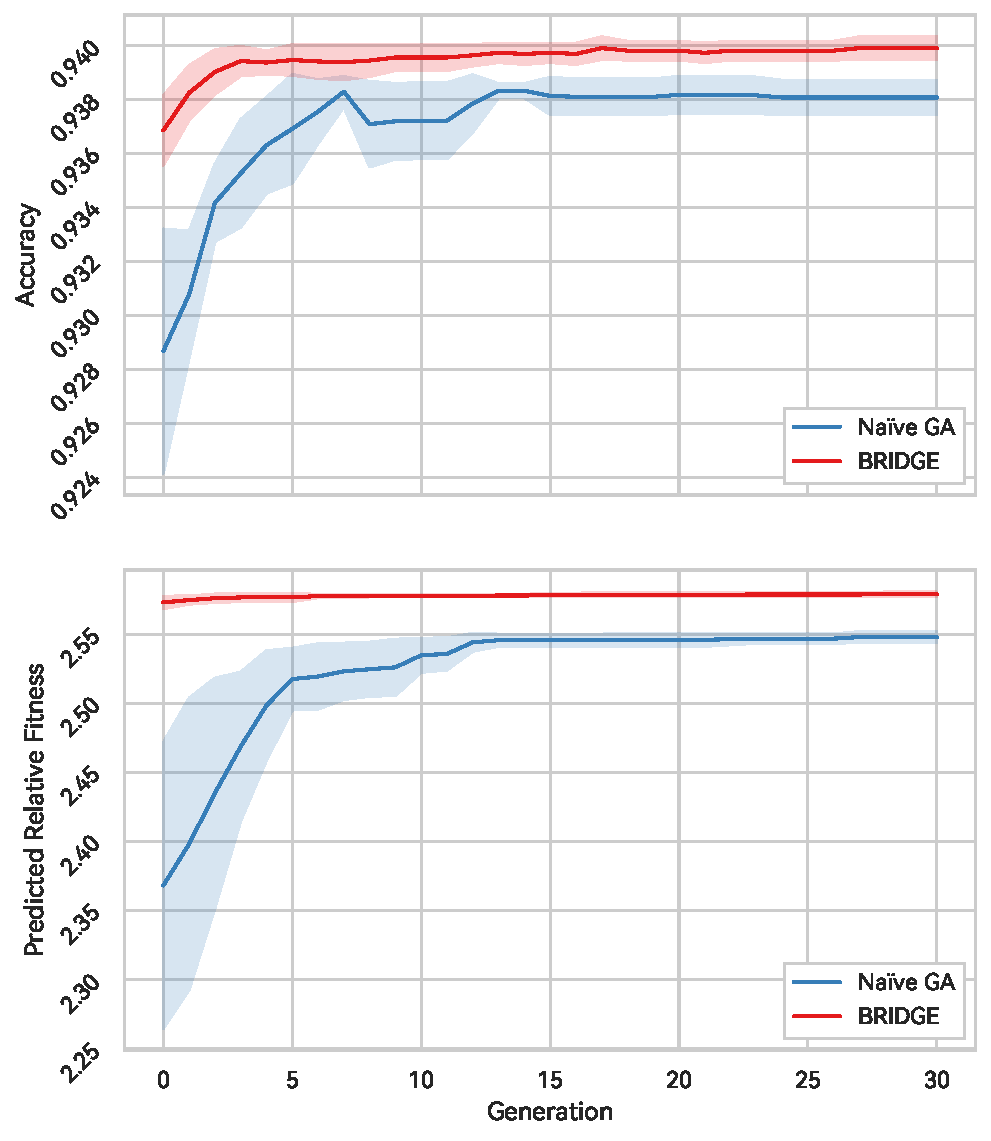
\includegraphics[width=.67\linewidth]{BRIDGE/search-plot.pdf}
	\bicaption[跨域ESTO性能对比]{在 NAS-Bench-101 上,有无 \textsc{Bridge} 跨域 ESTO 机制的进化神经架构搜索性能对比分析。
		\ \textit{上图:} 每代探索架构的真实准确率变化趋势。
		\ \textit{下图:} 排序模块预测的相对适应度分数,用于指导 NAS 过程作为评估策略。
	}[ESTO transfer performance]{
		Performance comparison of evolutionary NAS on NAS-Bench-101 with and without the \textsc{Bridge} cross-domain ESTO mechanism.
		\ \textit{Top:} evolution of true accuracy for architectures explored in each generation.
		\ \textit{Bottom:} relative fitness scores predicted by the ranking module that guide the NAS process as the evaluation strategy.
	}\label{fig:search-process-plot}
\end{figure}

我们通过从简单域向复杂域迁移的实验对所提方法进行了初步验证,具体利用 NAS-Bench-201 空间中的解来增强 NAS-Bench-101 空间的搜索。映射矩阵 \( \mathcal{M} \) 通过分别从两侧训练集中采样 1,000 个解构建而成。

我们选取遗传算法(Genetic Algorithm, GA)~\cite{geneticalgorithms_holland_1992} 作为进化搜索求解器,该方法在 NAS 中被广泛使用。参照~\cite{efficienttwostage_hou_2021} 的设置,GA 求解器采用种群规模 20,使用 \textit{单点交叉} 和 \textit{多项式变异}(概率均为 0.5),以及 \textit{二元锦标赛选择}。

结果如表~\ref{tab:transfer-result-101} 所示,与未采用所提跨域迁移方法的相同 GA 求解器(朴素 GA)基线相比,我们的方法取得了显著性能提升:最优准确率达 94.17\%,平均准确率达 93.99\%,大幅优于基线指标。对 10 次独立实验的统计分析证实了这些改进的显著性。

为进一步说明迁移学习对搜索过程的影响,图~\ref{fig:search-process-plot} 展示了种群最优解随代际的变化趋势。在早期阶段,迁移而来的解构建了高质量且多样化的初始种群,从而使得搜索从一开始就探索更优的解区域。综上所述,我们提出的迁移学习方法有效加速了神经架构搜索过程,使其更早收敛至更优结果区域。

此外,我们的迁移机制在进化计算框架内明确设计为求解器无关,强调其在不同优化方法中的广泛适用性。框架的模块化架构便于与现有 NAS 方法无缝集成,为多种搜索策略下的架构优化提供增强潜力。

为严格验证这种通用性,我们在表~\ref{tab:transfer-result-101} 中展示了与两种先进进化方法的集成实验:来自 EPCNAS~\cite{splitlevelevolutionary_huang_2023} 的 \textit{粒子群优化}(PSO)和来自 MSNAS~\cite{cellbasedfast_dong_2023} 的 \textit{模因算法}(MA)。实验结果表明,PSO 和 MA 分别比其基线实现提升了 0.19\% 和 0.25\%。重要的是,这些提升是在减少计算开销(更少的评估次数和迭代轮次)的前提下实现的。这些发现为框架的求解器无关性及其增强多种进化优化策略的能力提供了有力实证。

\mysubsection{向更具挑战性的域迁移}
\label{sec:ch4-8-4-transfer-to-challenging-domains}

为评估我们迁移学习框架的泛化能力,我们在 DARTS 架构空间中开展了大量实验,该空间在搜索域复杂度上显著提升。与 NAS-Bench-101 和 NAS-Bench-201 相比,DARTS 空间展现出显著的架构异质性,表现为操作词汇表扩展、每单元操作密度增加以及双单元类型配置。这些架构差异对知识迁移提出了重大挑战,为我们的方法提供了严格的验证框架。

我们的实验方案聚焦于从 NAS-Bench-101 域向 DARTS 搜索空间的知识迁移。我们保持与第~\ref{sec:nb101-exp} 节一致的超参数配置。实验流程包括预测器引导的收敛搜索,随后对基于 CIFAR-10 上预测性能指标选出的前 10 个架构进行全面训练。在完整训练阶段,我们遵循既定方法协议~\cite{regularizedevolutionimage_real_2019,learningtransferablearchitectures_zoph_2018,efficientneuralarchitecture_pham_2018,dartsdifferentiablearchitecture_liu_2019,cellbasedfast_dong_2023},实施了数据增强和 \textit{cutout} 增强技术。

表~\ref{tab:transfer-result-301} 总结了我们的方法与基线方法的性能对比。诸如 DARTS(97.24\%,耗时 4 GPU 天)和 MSNAS(97.32\%,耗时 0.23 GPU 天)等方法表明:高效的搜索机制可显著降低资源消耗。当引入迁移学习后(如 EMT-NAS 和 MTNAS,均采用 EA\,+\,TL 策略),模型在性能和成本上均获得进一步增益。

我们提出的方法 \textsc{Bridge} 同样采用 EA\,+\,TL 策略,在仅 0.21 GPU 天的搜索成本下达到了最高的准确率(97.33\%\,\(\pm\)\,0.06)。该结果不仅优于朴素 GA 基线(96.62\%,0.3 GPU 天),还在 DARTS 搜索空间中通过将高质量解从简单域有效迁移到复杂域,树立了新基准。

这些结果凸显了我们方法对多样化复杂架构设计的适应能力。这种适应性对于应对大规模搜索空间带来的挑战至关重要,从而验证了我们框架在现实场景中的实际适用性。此外,跨高异质性域的成功迁移表明,我们的表征学习方法能有效提取神经架构的底层语义信息。这种弥合差异域的能力有望显著推动自动机器学习领域的发展,实现跨任务、跨域的高效架构发现。

\begin{table}
	\centering
	\bicaption[DARTS空间性能对比]{在 CIFAR-10 上使用 DARTS 搜索空间与当前最先进 NAS 模型的对比}[DARTS comparison]{Comparison of the DARTS search space on CIFAR-10 with current state-of-the-art NAS models}\label{tab:transfer-result-301}

	\small\begin{NiceTabularX}{\textwidth}{p{9em}X[c]X[c]l}[notes,tabularnote={EA = 进化算法, RL = 强化学习, GD = 基于梯度, TL = 迁移学习。}]

		\toprule
		方法                                             & \Block{1-1}{平均准确率~(\%)} & \Block{1-1}{搜索成本 (GPU 天)} & \Block{1-1}{方法类型} \\
		\midrule\midrule
		ResNet-110~\cite{deepresiduallearning_he_2016}         & 93.40                        & --                             & 手动设计              \\
		DenseNet-BC~\cite{denselyconnectedconvolutional_huang_2017}     & 96.54                        & --                             & 手动设计              \\
		\midrule
		AmoebaNet-A~\cite{regularizedevolutionimage_real_2019}      & 96.66 \(\pm\) 0.06           & 3150                           & EA                    \\
		ENAS~\cite{efficientneuralarchitecture_pham_2018}                  & 97.11                        & 0.5                            & RL                    \\
		NAO~\cite{neuralarchitectureoptimization_luo_2018}              & 97.02                        & 200                            & GD                    \\
		DARTS~\cite{dartsdifferentiablearchitecture_liu_2019}              & 97.24 \(\pm\) 0.09           & 4                              & GD                    \\
		MSNAS~\cite{cellbasedfast_dong_2023}       & 97.32 \(\pm\) 0.08           & 0.23                           & EA                    \\
		\midrule
		EMT-NAS~\cite{emtnastransferring_liao_2023}           & 97.04 \(\pm\) 0.04           & 0.42                           & EA + TL               \\
		MTNAS~\cite{evolutionarymultitaskconvolutional_zhou_2024}       & 97.25 \(\pm\) 0.04           & 0.25                           & EA + TL               \\
		\midrule
		朴素~GA~(基线)                                   & 96.62 \(\pm\) 0.15           & 0.3                            & EA                    \\
		\textsc{Bridge}~(本文)                           & \textbf{97.33} \(\pm\) 0.06  & \bfseries 0.21                 & EA + TL               \\
		\bottomrule
	\end{NiceTabularX}
\end{table}

\mysection{深入分析}
\label{sec:ch4-9-in-depth-analysis}

\mysubsection{潜在表征空间观察}\label{sec:ch4-9-1-latent-embedding-space-observation}

为更直观地展示表征学习过程中潜在表征空间内分布的演化,我们采用 \textit{多维尺度分析}(Multi-Dimensional Scaling, MDS)~\cite{chapter3multidimensional_douglascarroll_1998} 进行可视化。此外,我们根据采样点的真实标签进行颜色编码,以辅助解读。

如图~\ref{fig:nb101-mds} 所示,在表征学习的不同阶段,具有相似性能指标的神经架构在潜在表征空间中表现出空间邻近性。这种聚集现象在训练过程中呈现出逐步增强的连贯性。

所观察到的聚类行为与 VAE 的固有特性一致。在预训练阶段,VAE 自然倾向于将相似的神经架构在潜在空间中置于邻近位置。此外,结构相似的架构更可能表现出相近的性能特征。这种内在组织为后续性能排序器的训练提供了坚实基础。在微调阶段,引入源自真实标签的监督信号进一步增强了模型捕捉影响性能差异特征的能力。这种优化反映在潜在空间分布中:具有相似性能指标的架构表征展现出显著的聚集性。

此外,我们将架构种群的进化动态映射到潜在空间中,如图~\ref{fig:nb101-mds-trace} 所示,说明迁移学习如何加速进化过程。通过利用 \textsc{Bridge},我们以高质量、多样化的解初始化种群,显著提升收敛速度,并发现先前未见的高性能解。

\begin{figure}[htbp]
	\centering
	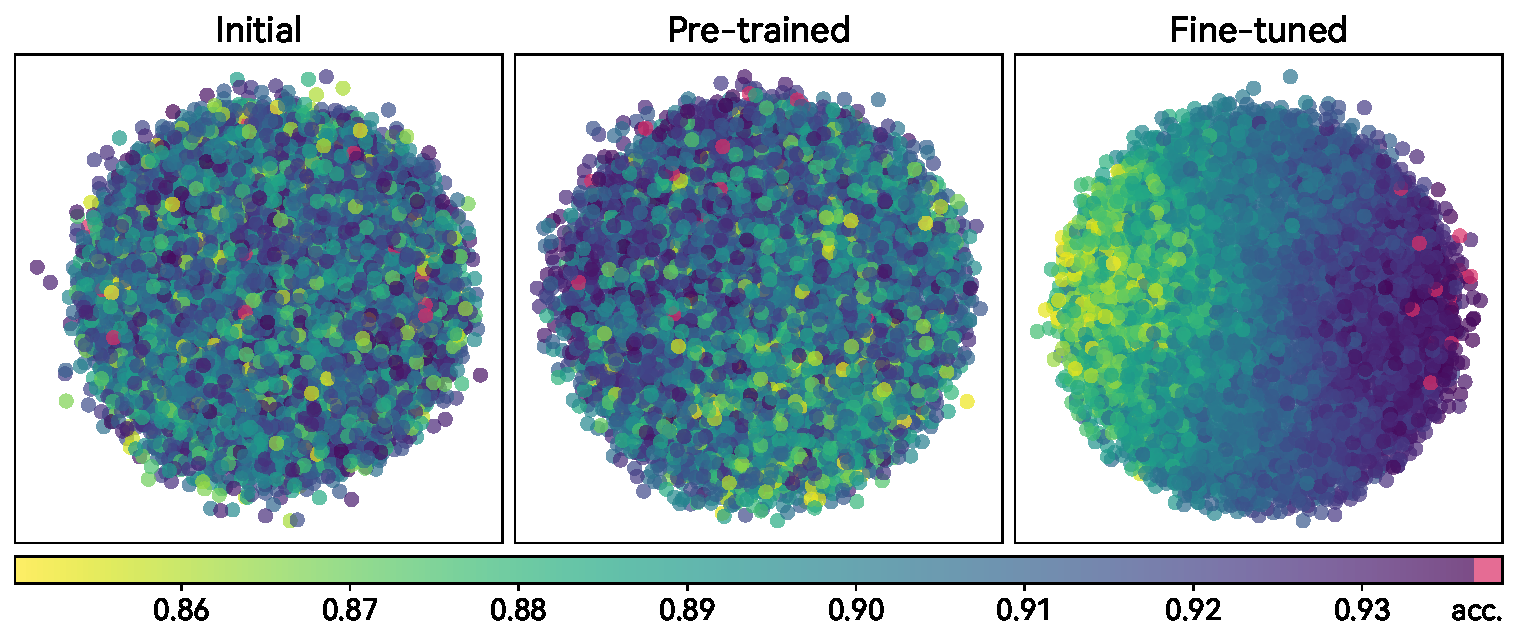
\includegraphics[width=.7\linewidth]{BRIDGE/nb101-mds.pdf}
	\bicaption[表征空间可视化]{NAS-Bench-101 架构在不同训练阶段的表征空间可视化:初始(左)、预训练后(中)和微调后(右)。
		颜色表示架构性能(准确率),暖色代表更高准确率。
	}[Representation space visualization]{Visualization of NAS-Bench-101 architectures in the representation space at different training stages: initial (left), after pre-training (middle), and after fine-tuning (right). Colors denote accuracy, with warmer tones indicating higher accuracy.}\label{fig:nb101-mds}
\end{figure}

\begin{figure}[htbp]
	\centering
	\includegraphics[width=.5\linewidth]{BRIDGE/nb101-mds-trace.pdf}
	\bicaption[进化动态对比]{NAS-Bench-101 上有无迁移学习的进化动态对比。
		图中比较了有迁移学习(右)和无迁移学习(左)时在 NAS-Bench-101 上的优化轨迹。
		轨迹通过每 10 代追踪最优解进行可视化。
	}[Evolution dynamics comparison]{Comparison of evolutionary dynamics on NAS-Bench-101 with and without transfer learning. The optimization trajectories are shown by tracking the best solution every 10 generations, with transfer learning on the right and the vanilla setting on the left.}\label{fig:nb101-mds-trace}
\end{figure}

\mysubsection{训练数据量的影响}
\label{sec:ch4-9-2-training-data-impact}

如第~\ref{sec:method-build-repre} 节所述,我们的表征学习框架采用两阶段训练策略:无监督预训练后接监督微调。该策略既能全面捕捉架构特性,又保持跨域可迁移性。

鉴于表征学习模型是所提迁移框架的基石,其有效性直接影响知识迁移能力和最终性能。所学表征的质量从根本上依赖于训练数据的规模与分布。为系统探究这一关系,我们开展了全面的实证研究,考察数据集规模对表征学习性能的影响。该分析为我们的方法在不同数据可用条件下的可扩展性与鲁棒性提供了关键洞见。

表~\ref{tab:ablation-pretrain-data-size} 展示了 NAS-Bench-101 数据集不同比例下预训练阶段的关键性能指标,特别分析了两个核心指标:VAE 重建准确率和计算开销(以 GPU 天计)。实验结果揭示了架构表征学习中的两个关键模式:1)模型性能与训练数据量呈强正相关,直至达到数据集 10\% 规模,此时 VAE 准确率达近完美的 99.91\%,且计算开销极低(0.08 GPU 天);2)超过该阈值后,数据量增至 30\%(三倍)仅带来微乎其微的准确率提升(99.56\%),却导致计算成本增加 37.5\%。这些发现表明,即使在有限数据条件下,我们的框架也能学习到鲁棒的架构嵌入。这种在相对小数据集下的高效表征学习能力,为实际迁移学习应用(尤其在架构数据难以获取或计算成本高昂的场景)提供了坚实的实证基础。

\begin{table}
	\centering
	\bicaption[无标签数据量影响]{无标签数据量对无监督预训练的影响}[Unlabeled data ablation]{Impact of unlabeled data volume on unsupervised pre-training}\label{tab:ablation-pretrain-data-size}
	\newcommand*{\ablationfn}{\tabularnote{为消除预测器对实验的干扰,我们在不同数据规模下使用统一的性能预测器。}}
	\small\begin{NiceTabularX}{\linewidth}{p{12em}*{5}{>{\centering\arraybackslash}X}}
		\toprule
		\bfseries 无标签数据 & \bfseries 1\% & \bfseries 5\% & \bfseries 10\% & \bfseries 30\% & \bfseries 50\% \\
		\midrule\midrule
		\textbf{VAE 准确率} (\%)   & 78.82         & 89.46         & 99.91          & 99.56          & 99.97          \\
		\textbf{成本} (GPU 天)     & 0.08          & 0.08          & 0.08           & 0.11           & 0.15           \\
		\bottomrule
	\end{NiceTabularX}
\end{table}

在微调阶段,如表~\ref{tab:ablation-finetune-data-size} 所示,VAE 在不同数据规模下均表现出稳健性能,准确率至少达 99.90\%,表明即使数据有限,它也能一致地捕捉神经架构的底层结构。

这表明无监督学习能有效建模架构特征,不受数据量变化的显著影响。然而,预测器组件的性能对训练数据量更为敏感。随着数据集规模增大,K-Tau 持续提升,在数据集 5\% 规模时达到最大值 0.865,反映出更大规模数据集带来的更强预测能力。

这种敏感性不仅体现在预测准确率上,还影响所学表征空间的分布特性。我们的研究指出,更大规模的标注数据有助于构建更结构化、更有组织的表征空间,从而促进域间更精确映射函数的学习。这种改进的空间结构和更高的跨域映射精度直接提升了目标任务上的搜索性能。例如,在使用 5\% 总数据集时,我们在源域达到 97.36\% 的准确率,在目标域达到 94.32\%,体现了更大规模数据集对跨域迁移能力的益处。

\begin{table}
	\centering
	\bicaption[标注数据量影响]{标注数据量对微调与迁移学习的影响}[Labeled data ablation]{Impact of labeled data volume on fine-tuning and transfer learning}\label{tab:ablation-finetune-data-size}

	\small\begin{NiceTabularX}{\linewidth}{p{12em}*{3}{>{\centering\arraybackslash}X}}
		\toprule
		\bfseries 标注数据                & \bfseries 0.1\% & \bfseries 1\% & \bfseries 5\% \\
		\midrule\midrule
		\bfseries Kendall's \(\bm{\tau}\)-b & 0.738           & 0.848         & 0.865         \\
		\bfseries 成本 (GPU 天)            & 0.01            & 0.02          & 0.02          \\
		\textbf{最优结果}                  &                 &               &               \\
		\quad --- 作为源域 (\%)           & 96.56           & 97.33         & 97.36         \\
		\quad --- 作为目标域 (\%)         & 94.02           & 94.17         & 94.32         \\
		\bottomrule
	\end{NiceTabularX}
\end{table}

综上所述,尽管 VAE 对有限数据表现出鲁棒性,但性能预测器和迁移学习阶段显著受益于更大规模的数据集。这凸显了在迁移学习场景中数据获取与整理的重要性,尤其是在目标域标注数据有限的情况下优化性能。

\mysubsection{探索不同的映射方法}
\label{sec:ch4-9-3-exploring-mapping-methods}

如第~\ref{sec:method-mapping} 节所述,我们采用线性映射方法来桥接异构域间的表征空间。该选择基于两个关键考量:计算效率与方法透明性。线性映射提供了一种优雅的解决方案,使我们能在保持算法简洁的同时验证显式解迁移的基本概念。

我们的实证分析表明,所学表征在潜在空间中呈现出平滑、结构良好的分布,自然有利于通过线性变换实现跨域迁移。从理论角度看,我们的表征学习框架专门设计用于在连续潜在空间中对神经架构进行编码,其中架构相似性得以保留,即使使用线性映射也能实现有效的知识迁移。

为严格评估映射复杂度对迁移性能的影响,我们对线性与非线性映射方法进行了对比研究。如表~\ref{tab:mapping-ablation} 所示,两种方法取得了相当的性能指标,未观察到统计显著差异(\(p = 0.462 > 0.05\))。这一发现表明,所学表征的质量而非映射复杂度,是决定迁移成功的主要因素。

\begin{table}
	\centering
	\bicaption[映射方法对比]{从 NAS-Bench-201 到 NAS-Bench-101 迁移学习中不同映射方法的性能对比}[Mapping methods comparison]{Performance comparison of different mapping methods when transferring from NAS-Bench-201 to NAS-Bench-101}\label{tab:mapping-ablation}
	\newcommand*{\ttestFn}{\tabularnote{所有 p 值均基于 10 次独立实验,相对于线性映射方法计算。}}
	\small\begin{NiceTabularX}{\linewidth}{p{10em} *{3}{>{\centering\arraybackslash}X}@{}}
		\toprule
		\RowStyle[nb-rows=1,bold]{}
		方法               & \Block{1-1}{最优准确率~(\%)} & \Block{1-1}{平均准确率~(\%)} & P 值~\ttestFn{} \\
		\midrule\midrule
		无迁移             & 93.85                        & \(93.77 \pm 0.11 \)          & 7.19E-06        \\
		线性映射           & 94.17                        & \(93.99 \pm 0.08 \)          & --              \\
		非线性映射         & 94.09                        & \(93.97 \pm 0.06 \)          & 4.62E-01        \\
		\bottomrule
	\end{NiceTabularX}
\end{table}

\begin{table}
	\centering
	\bicaption[进化超参数分析]{从 NAS-Bench-201 到 NAS-Bench-101 迁移学习中进化超参数分析}[Evolutionary hyperparameters]{Analysis of evolutionary hyperparameters when transferring from NAS-Bench-201 to NAS-Bench-101}\label{tab:esto-hyperparam-analysis}

	\small\begin{NiceTabularX}{\linewidth}{p[l]{8em} *{6}{>{\centering\arraybackslash}X}}[notes,tabularnote={\textbf{GA} 表示基线朴素 GA,而 \textbf{TL} 表示所提出的 \textsc{Bridge}。}]
		\toprule
		\RowStyle[nb-rows=1,bold]{}
		\Block{2-1}{参数范围} & \Block{1-2}{种群大小}          &       & \Block{1-2}{交叉概率}         &       & \Block{1-2}{变异概率}          &       \\
		{}                    & \Block{1-2}{\numlist{10;20;30}} &       & \Block{1-2}{\numrange{0.1}{0.9}} &       & \Block{1-2}{\numrange{0.1}{0.9}} &       \\
		\midrule\midrule
		\RowStyle[nb-rows=1,bold]{}
		{}                    & GA                              & TL    & GA                               & TL    & GA                               & TL    \\
		\midrule
		\textbf{相关性}       & 0.460                           & 0.629 & 0.374                            & 0.039 & 0.095                            & 0.527 \\
		\textbf{重要性}       & 0.287                           & 0.754 & 0.447                            & 0.051 & 0.267                            & 0.195 \\
		\bottomrule
	\end{NiceTabularX}
\end{table}

\mysubsection{超参数敏感性分析}\label{sec:ch4-9-4-hyperparameter-sensitivity}

基于 Transformer 的架构引入了若干关键超参数,这些参数显著影响表征学习效果。通过理论分析与文献回顾,我们确定注意力头数、嵌入维度和网络深度对所学表征质量具有特别强的影响。

我们进一步扩展分析,对这些参数进行了详细评估,结果表明:随着模型规模增大,超参数对表征学习性能的影响逐渐减弱。

我们对若干超参数候选值进行了网格搜索,包括 Transformer 层数(2、3、4)、模型维度(64、128)和自注意力头数(2、4、8)。实验结果显示,不同超参数配置下 VAE 准确率的标准差为 \(10^{-2}\);对于层数 ≥3 的配置,标准差降至 \(3 \times 10^{-3}\)。

图~\ref{fig:hyperparam-sensitivity} 中的平行坐标图进一步可视化了这些发现。

此外,我们对 \textsc{Bridge} 中进化搜索组件的超参数选择进行了系统研究。如表~\ref{tab:esto-hyperparam-analysis} 所示,我们探索了由种群大小(10、20、30)、交叉概率(0.1–0.9)和变异概率(0.1–0.9)定义的超参数空间。

为评估这些超参数对性能的影响,我们采用了两个互补指标:相关性与重要性。相关性通过 \textit{皮尔逊相关系数} 量化超参数与性能间的线性关系;重要性则通过训练随机森林回归器评估,以超参数为输入特征、性能指标为目标变量,其特征重要性得分揭示了非线性关系。

\textbf{种群大小。}
相关性从 GA 的 0.460 提升至 TL 的 0.629,重要性从 0.287 显著增至 0.754。这表明在 TL 中种群大小更为关键,可能源于迁移后对新搜索空间的探索与适应需求增强,促进了多样性与搜索效能。

\textbf{交叉概率。}
相关性从 GA 的 0.374 降至 TL 的 -0.039,重要性从 0.447 降至 0.051。这表明在 TL 中交叉操作影响减弱。虽然在 GA 中交叉有助于探索解空间,但在 TL 中,迁移知识已提供高质量、多样化的初始种群,降低了对交叉的依赖。

\textbf{变异概率。}
相关性从 GA 的 0.095 增至 TL 的 0.527,表明在 TL 中更高变异率更有利于探索新域,增强多样性并防止早熟收敛。然而,重要性从 0.267 降至 0.195。尽管相关性提升,但变异在 TL 中的相对贡献低于 GA,因为知识迁移已提供更优起点,减少了对变异进行初始发现的依赖。

综上所述,在 TL 中种群大小和变异概率比在 GA 中更为关键,需更大、更多样化的种群以适应新任务。交叉影响的减弱表明有效的知识迁移提供了强起点,降低了对交叉驱动探索的需求。这支持了 \textsc{Bridge} 在异构域间实现高质量、多样化知识迁移的能力。

\begin{figure}
	\centering
	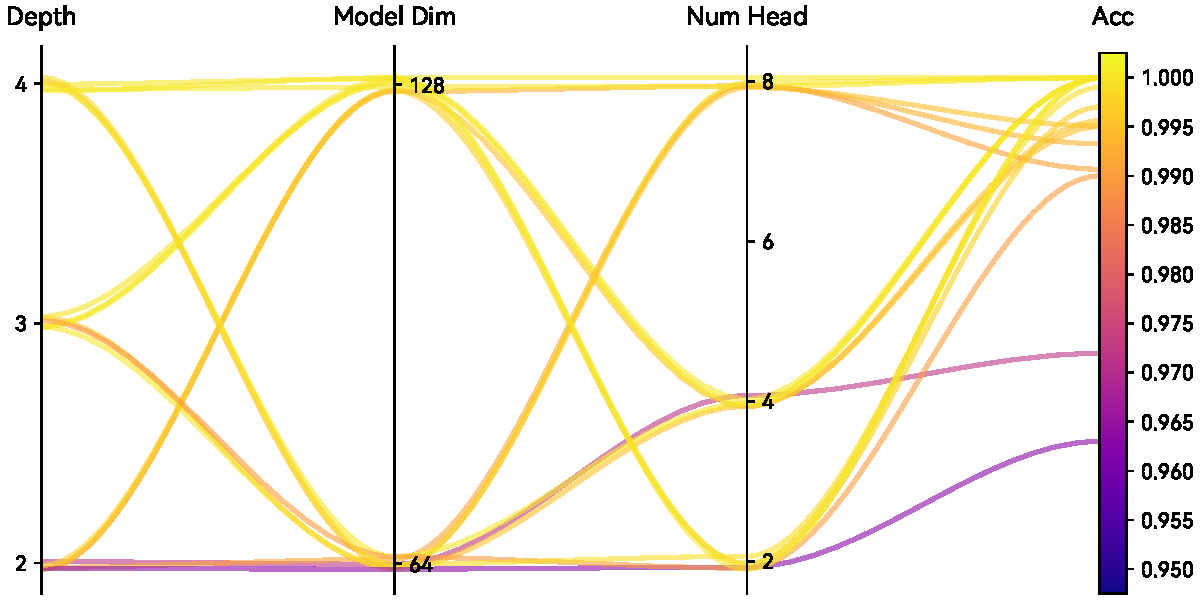
\includegraphics[width=.8\linewidth]{BRIDGE/hpsa.pdf}
	\bicaption[超参数敏感性分析]{
		平行坐标图展示了 NAS-Bench-101 上不同超参数设置下所提表征学习器的准确率。
		每条线对应网络深度、模型维度和注意力头数的一种唯一组合,颜色尺度表示所得准确率(深色线表示较低准确率,亮色线表示较高准确率)。
	}[Hyperparameter sensitivity analysis]{
		Parallel coordinates plot showing the accuracy of the proposed representation learner on NAS-Bench-101 under different hyperparameter settings.
		Each line corresponds to a unique combination of network depth, model dimension, and number of attention heads, with color indicating the resulting accuracy (darker lines for lower accuracy, brighter lines for higher accuracy).
	}\label{fig:hyperparam-sensitivity}
\end{figure}

\mysection{本章小结}\label{sec:ch4-10-chapter-summary}

本章聚焦于深度模型结构层面的高效构建挑战,特别是针对神经架构搜索中存在的计算成本高昂以及架构知识难以跨越异构搜索空间进行复用的核心瓶颈。为应对这一挑战,本文提出并详细阐述了一种名为 \textsc{Bridge} 的新型跨域进化迁移神经架构搜索框架。

\textsc{Bridge} 框架的核心创新在于其解决异构迁移难题的独特思路:它并非直接迁移架构的句法结构,而是通过引入统一的神经架构表示学习机制,将来自不同搜索空间(具有不同操作集、拓扑规则和编码方式)的架构映射到一个共享的、结构感知的潜在语义空间。在此基础上,框架进一步学习了一个跨域表示映射函数,以显式地桥接源域与目标域之间的表示差异,使得源域的高性能架构解能够在目标域中找到语义上对应的表示。最终,通过将这些迁移而来的高质量表示解码为目标域架构,并将其作为进化序贯迁移优化策略的初始种群,\textsc{Bridge} 实现了源域知识的高效引导与目标域架构的自适应进化相结合。

本章详细介绍了 \textsc{Bridge} 框架的各个关键技术组件,包括定制化的神经架构分词器、基于 Transformer 的变分自编码器(用于表示学习)、基于性能排序的映射学习方法以及 ESTO 算法的具体实现。通过在一系列复杂度递增的标准 NAS 基准(NAS-Bench-101, NAS-Bench-201, DARTS)上进行的大量实验验证,结果表明:(1) 所提出的架构表示学习方法能够有效地捕捉架构的关键特征并与性能相关联;(2) \textsc{Bridge} 框架能够成功地实现跨越显著异构的搜索空间(例如从 NAS-Bench-201 到 NAS-Bench-101,从 NAS-Bench-101 到 DARTS)的知识迁移;(3) 与不使用迁移的基线 NAS 方法或其他 TNAS 方法相比,\textsc{Bridge} 能够在显著降低搜索成本(例如,平均减少约 50\% 的 GPU 评估时间)的同时,发现性能相当甚至更优的神经网络架构。

综上所述,本章提出的 \textsc{Bridge} 框架为解决跨异构搜索空间的神经架构知识迁移这一前沿挑战提供了一种有效且可行的解决方案。通过结合先进的表示学习技术与进化迁移优化策略,\textsc{Bridge} 不仅显著提升了 NAS 的效率和通用性,也为自动化机器学习领域中更广泛的知识复用与迁移问题提供了新的思路和启示。

\end{document}
